\documentclass[12pt,a4paper]{article}
% PACKAGES 
\usepackage{amsmath,amsfonts,amssymb}
\usepackage{graphicx}
\usepackage{enumitem}
\usepackage[dvipsnames]{xcolor}
\usepackage{pgfplots}
\usepackage{hyperref}
\usepackage{soul}
\usepackage{framed}
\usepackage{booktabs} 
\usepackage{tabularx}
\usepackage{array}
\usepackage{adjustbox}
\usepackage{mathtools}
\usepackage{siunitx}
\usepackage{subcaption}
\usepackage{tikz}
\usepackage{float}
\usepackage{cancel}
\usepackage{booktabs} 
\usepackage{array}
\usepackage{tcolorbox}
\usepackage{amsmath, amssymb, amsthm}
\usepackage{xcolor}
\usepackage[utf8]{inputenc}
\usepackage{physics}
\usepackage[outline]{contour} % glow around text
\contourlength{1.3pt}
\usepackage[amsmath]{empheq}
\usepackage{titlesec}
\usepackage[x11names,svgnames,dvipsnames]{xcolor}

% USETIKZLIBRARY
\usetikzlibrary{arrows.meta}
\usetikzlibrary{angles, arrows.meta, quotes}
\usetikzlibrary{arrows}
\usetikzlibrary{shapes}
\usetikzlibrary{3d, shapes.multipart}


\newcommand{\mymk}[1]{%
  \tikz[baseline=(char.base)]\node[anchor=south west, draw,rectangle, rounded corners, inner sep=2pt, minimum size=7mm,
    text height=2mm](char){\ensuremath{#1}} ;}

\newcommand*\circled[1]{\tikz[baseline=(char.base)]{
            \node[shape=circle,draw,inner sep=2pt] (char) {#1};}}


\renewcommand{\arraystretch}{1.5}
\setlength{\tabcolsep}{12pt}

\newlist{arrowlist}{itemize}{1}
\setlist[arrowlist]{label=$\Rightarrow$}

\definecolor{lessonbgcolor}{rgb}{0.9,0.9,1}
\definecolor{examplecolor}{rgb}{0.8,1,0.8}
\definecolor{noteboxcolor}{rgb}{1,0.8,0.8}
\newenvironment{lesson}[1]
  {\begin{framed}\colorbox{lessonbgcolor}{
  \parbox{\dimexpr\linewidth-2\fboxsep}{
  \textbf{#1}}}\end{framed}}
  
\newenvironment{example}
  {\begin{framed}\colorbox{examplecolor}{
  \parbox{\dimexpr\linewidth-2\fboxsep}{
  \textbf{Example:}}}}
  {\end{framed}}
\newenvironment{note}
  {\begin{framed}\colorbox{noteboxcolor}{
  \parbox{\dimexpr\linewidth-2\fboxsep}{
  \textbf{Note:}}}}
  {\end{framed}}
\newenvironment{GS}[1]
{\subsection*{#1}\begin{minipage}{0.9\linewidth}\raggedright}
{\end{minipage}}  



\definecolor{shadecolor}{cmyk}{0,0,0.45,0}
\definecolor{light-blue}{cmyk}{0.25,0,0,0}
\newsavebox{\mysaveboxM}
\newsavebox{\mysaveboxT}
\newcommand*\Garybox[2][Log law]{%
  \sbox{\mysaveboxM}{#2}%
  \sbox{\mysaveboxT}{\fcolorbox{black}{light-blue}{#1}}%
  \sbox{\mysaveboxM}{%
    \parbox[b][\ht\mysaveboxM+0.5\ht\mysaveboxT+0.5\dp\mysaveboxT][b]{%
      \wd\mysaveboxM}{#2}%
  }%
  \sbox{\mysaveboxM}{%
    \fcolorbox{black}{shadecolor}{%
      \makebox[\linewidth-17.5em]{\usebox{\mysaveboxM}}%
    }%
  }%
  \usebox{\mysaveboxM}%
  \makebox[0pt][r]{%
    \makebox[\wd\mysaveboxM][c]{%
      \raisebox{\ht\mysaveboxM-0.5\ht\mysaveboxT
                +0.5\dp\mysaveboxT-0.5\fboxrule}{\usebox{\mysaveboxT}}%
    }%
  }%
}
\definecolor{darkgreen}{RGB}{0, 100, 0}
  

\pgfplotsset{width=7cm,compat=1.17}

\pgfplotsset{width=7cm,compat=1.17}


%COLORLET
\colorlet{veccol}{green!70!black}
\colorlet{vcol}{green!70!black}
\colorlet{xcol}{blue!85!black}
\colorlet{projcol}{xcol!60}
\colorlet{unitcol}{xcol!60!black!85}
\colorlet{unitcol2}{vcol!60!black!85}
\colorlet{myblue}{blue!70!black}
\colorlet{myred}{red!70!black}
\def\tick#1#2{\draw[thick] (#1) ++ (#2:0.1) --++ (#2-180:0.2)} %0.03*\xmax


% Define colors
\definecolor{myblue}{RGB}{0, 0, 255}
\definecolor{mygreen}{RGB}{0, 128, 0}

% Set up theorem environments
\newtheorem{theorem}{Theorem}[section]
\newtheorem{definition}{Definition}[section]


% Set up section and subsection headings with color

\titleformat{\section}{\color{myblue}\normalfont\Large\bfseries}{\thesection}{1em}{}
\titleformat{\subsection}{\color{mygreen}\normalfont\large\bfseries}{\thesubsection}{1em}{}


\newcommand{\trigfuns}[3][1]% #1 is scale factor (default=1), #2 is angle
    {\begin{tikzpicture}[scale=#1, semithick, every node/.style={circle, inner sep=.1mm, font=\scriptsize}]
        \draw (0,0) circle[radius=1];
        \draw (0,0) -- (#2:{max(sec(#2),cosec(#2))});
        \draw (0,0) -- (0,1) -- ({cot(#2)},1)node [label={[above, midway]$\theta$}] {};
        \draw (0,0) -- (1,0) -- (1,{tan(#2)})node [label={[right, midway]$w$}] {};
        \draw ({cos(#2)},0) -- ({cos(#2)},{sin(#2)})node [label={[left,midway]$s$}] {} 
            -- (0, {sin(#2)})node [label={[above,midway]$t$}] {};
        \node at ({.5*cos(#2)},{.5*sin(#2)}) [label=#2+90:$1$] {}; 
        \draw (0:.3) arc (0:#2:.3)node [label={[yshift=.3mm,right,midway]$#3$}] {};
    \end{tikzpicture}}



% Define custom colors
\definecolor{myblue}{RGB}{70,130,180}

% Create a box style for highlights
\tcbset{
    mybox/.style={
        colframe=myblue,
        colback=white,
        sharp corners,
        boxrule=1pt,
        left=0pt,
        right=0pt,
        top=0pt,
        bottom=0pt
    }
}




\title{Grade 11 Functions Notes}
\author{Made By Kensukeken}
\date{30, January 2023}

\begin{document}
\maketitle
\tableofcontents
\newpage
\section{Unit 1: Intro To Functions}

\subsection{Lesson 1 - Domain and Range}
The domain and range of a function describe the possible input and output values, respectively.



\textbf{\hl{Example 1:}} For \(f(x) = \sqrt{x}\), the domain is \(x \geq 0\) since you can't take the square root of a negative number without delving into complex numbers.

\textbf{\hl{Example 2:}} For \(f(x) = \frac{1}{x}\), the domain is \(x \neq 0\) since division by zero is undefined.

\textbf{\hl{Example 3:}} For a parabola \(f(x) = x^2\), the range is \(f(x) \geq 0\).

\subsection*{Lesson 2 - Function Notation}
Function notation introduces a more concise way to represent equations.

\textbf{\hl{Example 1:}} Given \(f(x) = 2x^2 + 3\), find \(f(2)\). Solution: \(f(2) = 2(2^2) + 3 = 11\).

\textbf{\hl{Example 2:}} If \(f(x) = x + 5\), what is \(f(3)\)? Solution: \(f(3) = 3 + 5 = 8\).

\textbf{Function Table for \(f(x) = x^2\)}:
\begin{center}
    \begin{tabular}{c|c}
        \( x \) & \( f(x) \) \\
        \hline
        -2 & 4 \\
        -1 & 1 \\
        0 & 0 \\
        1 & 1 \\
        2 & 4 \\
    \end{tabular}
\end{center}
\newpage
\subsection{Lesson 3 - Max/Min of Quadratics}
The vertex of a quadratic function indicates its maximum or minimum value.
\subsubsection*{Properties of Quadratic Expressions}

Quadratic expressions, depending on their leading coefficients, have certain inherent properties:

\begin{enumerate}
    \item Any square of a number, \(x^2\), is always non-negative. Thus, \(x^2 \geq 0\). This is because squaring any real number, whether positive or negative, results in a positive value (or zero if \(x = 0\)).
    
    \item The negative of a square, \(-x^2\), is always non-positive. Thus, \(-x^2 \leq 0\). This is the opposite behavior of \(x^2\), as negating it ensures the parabola opens downward.
    
    \item For a quadratic in the form of \(-(x-h)^2\), where \(h\) is a constant, the expression represents a downward-opening parabola shifted \(h\) units to the right on the x-axis. As an example, for \(-(x-4)^2\), the parabola is shifted 4 units to the right, and \(-(x-4)^2 \leq 0\).
\end{enumerate}

\textbf{Note:} The sign and nature of the leading coefficient in a quadratic expression can give insights into the orientation of the parabola and its range.

\textbf{\hl{Example 1:}} Find the vertex of \(f(x) = 2x^2 + 4x + 3\). By completing the square, the vertex is \((-1, 1)\).

\textbf{\hl{Example 2:}} For \(f(x) = -x^2 + 4x - 3\), the vertex is \((2, 5)\) and represents a maximum due to the negative leading coefficient.

\subsection*{Lesson 4 - Radicals}
Radicals involve taking roots of numbers.

\textbf{\hl{Example 1:}} Simplify \(\sqrt[3]{27}\). Solution: \(3\).

\textbf{\hl{Example 2:}} Simplify \(\sqrt{81}\). Solution: \(9\).

\textbf{\hl{Example 3:}} Determine the domain of \(f(x) = \sqrt{x - 5}\). Solution: \(x \geq 5\).

\subsection*{Lesson 5 - Solve Quadratics by Factoring}
Factoring is a method to solve quadratic equations.

\textbf{\hl{Example 1:}} Solve \(x^2 - 5x + 6 = 0\). Solution: \((x - 2)(x - 3) = 0\), so \(x = 2\) or \(x = 3\).

\textbf{\hl{Example 2:}} Solve \(x^2 - x - 6 = 0\). Solution: \((x - 3)(x + 2) = 0\), so \(x = 3\) or \(x = -2\).

\subsection{Lesson 6 - Quadratic Formula}
When factoring is not possible, the quadratic formula offers a solution.

\textbf{Formula:}
\[x = \frac{-b \pm \sqrt{b^2 - 4ac}}{2a}\]

\textbf{\hl{Example:}} Solve \(x^2 + x - 1 = 0\). Plugging the coefficients into the formula will give two solutions for \(x\).

\subsection{Lesson 7 - Linear Quadratic Systems}

Linear Quadratic Systems involve a combination of linear and quadratic equations. Solving these systems can reveal points of intersection between the two functions, if they exist.

\textbf{Methods of Solution:}
\begin{enumerate}
    \item \textbf{Substitution:} Use the linear equation to solve for \(y\) (or \(x\)), and then substitute this expression into the quadratic equation.
    \item \textbf{Graphical:} Graph both the linear and quadratic functions on the same set of axes and identify the point(s) of intersection.
\end{enumerate}

\textbf{\hl{Example 1:}} Solve the system:
\[
\begin{aligned}
    y &= x^2 + 2 \\
    y &= 2x + 3
\end{aligned}
\]

By substitution, set \(x^2 + 2\) equal to \(2x + 3\). Solving this equation will give the \(x\)-coordinates of the intersection points. To find the corresponding \(y\)-coordinates, substitute these \(x\)-values into either the linear or quadratic equation.

\textbf{\hl{Example 2:}} Solve the system:
\[
\begin{aligned}
    y &= x^2 - 4 \\
    y &= -x + 2
\end{aligned}
\]

Again, using substitution, equate \(x^2 - 4\) to \(-x + 2\). This will yield the \(x\)-coordinates of where the line intersects the parabola. To find the corresponding \(y\)-values, plug these \(x\)-values into one of the original equations.

\textbf{Note:} Sometimes, a linear function might not intersect a quadratic function, or it might intersect at one or two points. The nature of intersection can also be discerned graphically or by assessing the discriminant when setting the two equations equal to each other.

\subsection{Translations and Function Notation}

Given a function \( y = f(x) \), the following transformations can be applied:

\begin{itemize}
    \item \textbf{Vertical Translation:} \( y = f(x) + c \) shifts the graph \(c\) units upward (if \(c > 0\)) or downward (if \(c < 0\)).
    \item \textbf{Horizontal Translation:} \( y = f(x - h) \) shifts the graph \(h\) units to the right (if \(h > 0\)) or to the left (if \(h < 0\)).
    \item \textbf{Vertical Stretch/Compression:} \( y = af(x) \) stretches the graph by a factor of \(a\) if \(a > 1\), or compresses it if \(0 < a < 1\). If \(a < 0\), the graph is also reflected about the x-axis.
    \item \textbf{Horizontal Stretch/Compression:} \( y = f(bx) \) compresses the graph horizontally by a factor of \(b\) if \(b > 1\), or stretches it if \(0 < b < 1\).
\end{itemize}

A translation is a type of transformation that changes the location of a function in the coordinate plane, while preserving its shape and size.

\subsubsection{Representation Using Function Notation}
Translations can be represented using function notation:
\[ y = f(x - h) + k \]
This represents the function \( y = f(x) \) translated horizontally by \( h \) units and vertically by \( k \) units.

\begin{itemize}
    \item If \( h > 0 \), the function is translated to the right.
    \item If \( h < 0 \), the function is translated to the left.
    \item If \( k > 0 \), the function is translated up.
    \item If \( k < 0 \), the function is translated down.
\end{itemize}

\subsubsection*{Sketching Translated Graphs}
To sketch the graph of \( y = f(x - h) + k \), start with the graph of \( f(x) \) and translate points on that function based on the values of \( h \) and \( k \). Asymptotes, if any, must also be translated.

\subsubsection*{Translations of Common Base Functions}
\vspace*{\fill}
\[
\begin{tabular}{|c|c|}
    \hline
    \textcolor{Orchid}{Base Function} & \textcolor{WildStrawberry}{Translated Function} \\
    \hline
    \( f(x) = x^2 \) & \( y = (x - h)^2 + k \) \\
    \hline
    \( f(x) = \sqrt{x} \) & \( y = \sqrt{x - h} + k \) \\
    \hline    
    \( f(x) = \frac{1}{x} \) & \( y = \frac{1}{x - h} + k \) \\
    \hline
\end{tabular}
\]
\vspace*{\fill}

\subsubsection*{$\bigstar$ Domain and Range}
When a function is translated, the domain and range of the function are translated as well.

\subsection*{\textcolor{blue}{Examples}}

\textbf{\hl{Example 1:}} Consider the function \(y = \sqrt{x}\).

\textbf{Transformation:} The graph of \(y = 2\sqrt{x-3} + 1\):

\begin{itemize}
    \item Starts with the basic square root graph.
    \item Stretches vertically by a factor of 2.
    \item Translates 3 units to the right.
    \item Translates 1 unit upwards.
\end{itemize}

\textbf{Description:} This graph will resemble the basic upward curving square root graph, but will be steeper (due to the vertical stretch), and shifted to the point (3,1) as its starting point.

\textbf{\hl{Example 2:}} Consider the function \(y = x^2\).

\textbf{Transformation:} The graph of \(y = -0.5(x+2)^2 - 4\):

\begin{itemize}
    \item Starts with the basic parabolic graph.
    \item Reflects about the x-axis (due to the negative sign).
    \item Compresses vertically by a factor of 0.5.
    \item Translates 2 units to the left.
    \item Translates 4 units downward.
\end{itemize}

\textbf{Description:} This graph will resemble an upside-down parabola, opening downward, being wider than the standard \(y = x^2\) graph (due to the vertical compression), and having its vertex at the point (-2,-4).

\subsection*{\hl{Shortcut Words For Transformation}}
\begin{align*}
    & \text{\hl{VT}} \xrightarrow{} \text{Vertical Translation} \\
    & \text{\hl{HT}} \xrightarrow{} \text{Horizontal Translation} \\
    & \text{\hl{VS}} \xrightarrow{} \text{Vertical Stretch} \\
    & \text{\hl{HS}} \xrightarrow{} \text{Horizontal Stretch} \\
    & \text{\hl{RXA}} \xrightarrow{} \text{Reflection in x-axis} \\
    & \text{\hl{RYA}} \xrightarrow{} \text{Reflection in y-axis} \\
\end{align*}

\subsection*{Summary Lesson}

\[
\begin{array}{lll}
\text{Notation} & \text{Transformation Type} & \text{Coordinate Change} \\
\textcolor{CadetBlue}{f(x)+d} & \textcolor{CadetBlue}{\text{Vertical translation up } d \text{ units}} & (x, y) \mapsto(x, y+d) \\
\textcolor{CadetBlue}{f(x)-d} & \textcolor{CadetBlue}{\text{Vertical translation down } d \text{ units}} & (x, y) \mapsto(x, y-d) \\
\textcolor{CadetBlue}{f(x+c)} & \textcolor{CadetBlue}{\text{Horizontal translation left } c \text{ units}} & (x, y) \mapsto(x-c, y) \\
\textcolor{CadetBlue}{f(x-c)} & \textcolor{CadetBlue}{\text{Horizontal translation right } c \text{ units}} & (x, y) \mapsto(x+c, y) \\
\textcolor{CadetBlue}{-f(x)} & \textcolor{CadetBlue}{\text{Reflection over } x \text{-axis}} & (x, y) \mapsto(x,-y) \\
\textcolor{CadetBlue}{f(-x)} & \textcolor{CadetBlue}{\text{Reflection over } y \text{-axis}} & (x, y) \mapsto(-x, y) \\
\textcolor{CadetBlue}{a f(x)} & \textcolor{CadetBlue}{\text{Vertical stretch for } |a|>1} & (x, y) \mapsto(x, a y) \\
\textcolor{CadetBlue}{a f(x)} & \textcolor{CadetBlue}{\text{Vertical compression for } |a|<1} & (x, y) \mapsto(x, a y) \\
\textcolor{CadetBlue}{f(b x)} & \textcolor{CadetBlue}{\text{Horizontal compression for } |b|>1} & (x, y) \mapsto\left(\frac{x}{b}, y\right) \\
\textcolor{CadetBlue}{f(b x)} & \textcolor{CadetBlue}{\text{Horizontal stretch for } |b|<1} & (x, y) \mapsto\left(\frac{x}{b}, y\right)
\end{array}
\]


\newpage
\section*{\hl{Parent Functions}}

\subsection*{1. Linear Function: $f(x) = x$}
\begin{minipage}{0.5\textwidth}
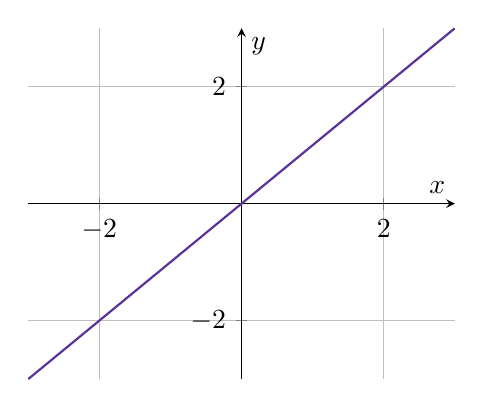
\begin{tikzpicture}
    \begin{axis}[
        grid=both,
        axis lines=middle,
        xmin=-3, xmax=3,
        ymin=-3, ymax=3,
        xlabel={$x$},
        ylabel={$y$},
        ]
        \addplot[RoyalPurple, thick, domain=-3:3] {x};
    \end{axis}
\end{tikzpicture}
\end{minipage}
\hspace{1cm}
\begin{minipage}{0.4\textwidth}
\centering
\begin{tabular}{cc}

$x$ & $f(x)$ \\
-2 & -2 \\
-1 & -1 \\
0 & 0 \\
1 & 1 \\
2 & 2 \\

\end{tabular}
\end{minipage}

The linear function $f(x) = x$ represents a \hl{straight line} that passes through the origin (0,0) and has a slope of 1. As $x$ increases or decreases, $f(x)$ increases or decreases respectively.

\subsection*{2. Quadratic Function: $f(x) = x^2$}
\begin{minipage}{0.5\textwidth}
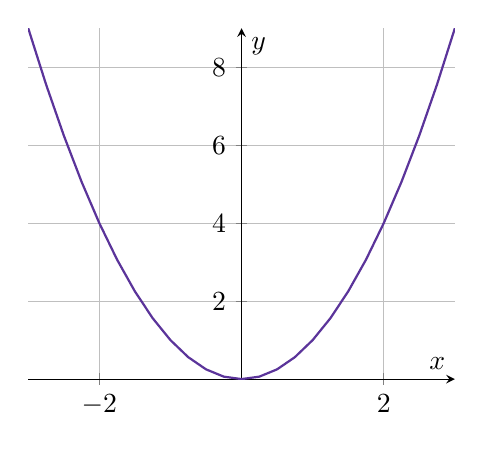
\begin{tikzpicture}
    \begin{axis}[
        grid=both,
        axis lines=middle,
        xmin=-3, xmax=3,
        ymin=0, ymax=9,
        xlabel={$x$},
        ylabel={$y$},
        ]
        \addplot[RoyalPurple, thick, domain=-3:3] {x^2};
    \end{axis}
\end{tikzpicture}
\end{minipage}
\hspace{1cm}
\begin{minipage}{0.4\textwidth}
\centering
\begin{tabular}{cc}
\toprule
$x$ & $f(x)$ \\

-2 & 4 \\
-1 & 1 \\
0 & 0 \\
1 & 1 \\
2 & 4 \\

\end{tabular}
\end{minipage}

The quadratic function $f(x) = x^2$ represents a parabola that opens upwards and has \hl{its vertex} at the origin (0,0). The function values are always non-negative and increase quadratically as $x$ moves away from 0.

\subsection*{3. Cubic Function: $f(x) = x^3$}
\begin{minipage}{0.5\textwidth}
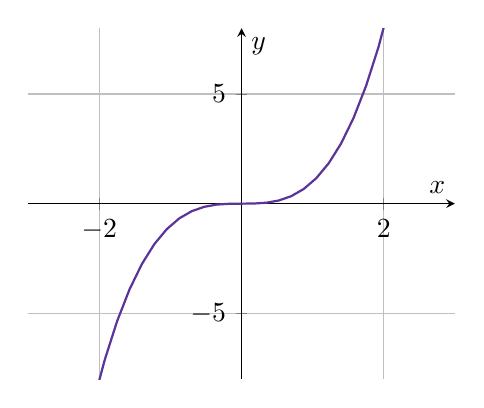
\begin{tikzpicture}
    \begin{axis}[
        grid=both,
        axis lines=middle,
        xmin=-3, xmax=3,
        ymin=-8, ymax=8,
        xlabel={$x$},
        ylabel={$y$},
        ]
        \addplot[RoyalPurple, thick, domain=-2.1:2.1] {x^3};
    \end{axis}
\end{tikzpicture}
\end{minipage}
\hspace{1cm}
\begin{minipage}{0.4\textwidth}
\centering
\begin{tabular}{cc}

$x$ & $f(x)$ \\

-2 & -8 \\
-1 & -1 \\
0 & 0 \\
1 & 1 \\
2 & 8 \\
\end{tabular}
\end{minipage}

The cubic function $f(x) = x^3$ has a characteristic \hl{S-shape} and crosses the origin (0,0). The function values increase cubically as $x$ moves away from 0, with $f(x)$ being negative when $x$ is negative and positive when $x$ is positive.

\subsection*{4. Reciprocal Function: $f(x) = \frac{1}{x}$}
\begin{minipage}{0.5\textwidth}
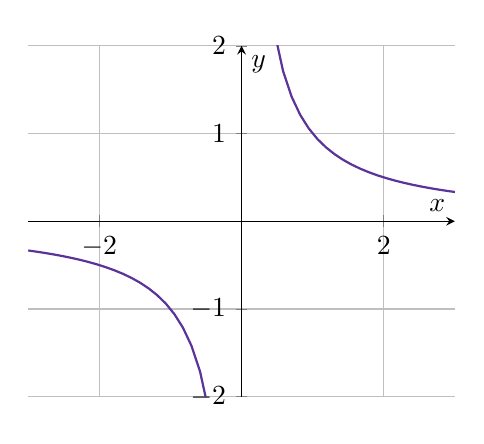
\begin{tikzpicture}
    \begin{axis}[
        grid=both,
        axis lines=middle,
        xmin=-3, xmax=3,
        ymin=-2, ymax=2,
        xlabel={$x$},
        ylabel={$y$},
        ]
        \addplot[RoyalPurple, thick, domain=-3:-0.1] {1/x};
        \addplot[RoyalPurple, thick, domain=0.1:3] {1/x};
    \end{axis}
\end{tikzpicture}
\end{minipage}
\hspace{1cm}
\begin{minipage}{0.4\textwidth}
\centering
\begin{tabular}{cc}

$x$ & $f(x)$ \\

-3 & -0.33 \\
-2 & -0.5 \\
-1 & -1 \\
1 & 1 \\
2 & 0.5 \\
3 & 0.33 \\

\end{tabular}
\end{minipage}
\noindent
The reciprocal function $f(x) = \frac{1}{x}$ has \hl{two hyperbolas} in the 1st and 3rd quadrants. As $x$ approaches 0 from either side, $f(x)$ approaches $\pm\infty$. 

\subsection*{5. Square Root Function: $f(x) = \sqrt{x}$}
\begin{minipage}{0.5\textwidth}
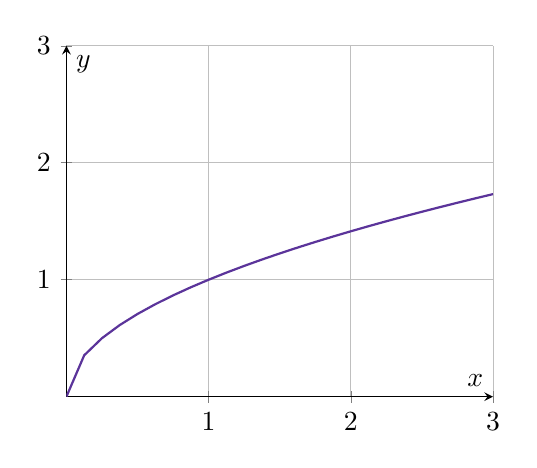
\begin{tikzpicture}
    \begin{axis}[
        grid=both,
        axis lines=middle,
        xmin=0, xmax=3,
        ymin=0, ymax=3,
        xlabel={$x$},
        ylabel={$y$},
        ]
        \addplot[RoyalPurple, thick, domain=0:3] {sqrt(x)};
    \end{axis}
\end{tikzpicture}
\end{minipage}
\hspace{1cm}
\begin{minipage}{0.4\textwidth}
\centering
\begin{tabular}{cc}
\toprule
$x$ & $f(x)$ \\

0 & 0 \\
1 & 1 \\
2 & 1.41 \\
3 & 1.73 \\

\end{tabular}
\end{minipage}
\noindent
The square root function $f(x) = \sqrt{x}$ is defined for $x \geq 0$ and represents \hl{half of a parabola} that opens upwards. As $x$ increases, $f(x)$ increases more slowly.


\subsection*{6. Absolute Value Function: $f(x) = |x|$}
\begin{minipage}{0.5\textwidth}
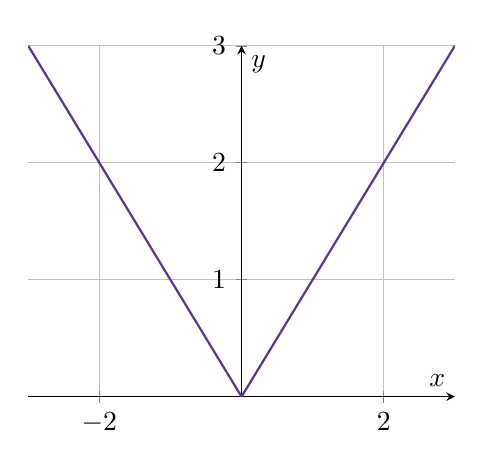
\begin{tikzpicture}
    \begin{axis}[
        grid=both,
        axis lines=middle,
        xmin=-3, xmax=3,
        ymin=0, ymax=3,
        xlabel={$x$},
        ylabel={$y$},
        ]
        \addplot[RoyalPurple, thick, domain=-3:3] {abs(x)};
    \end{axis}
\end{tikzpicture}
\end{minipage}
\hspace{1cm}
\begin{minipage}{0.4\textwidth}
\centering
\begin{tabular}{cc}

$x$ & $f(x)$ \\

-2 & 2 \\
-1 & 1 \\
0 & 0 \\
1 & 1 \\
2 & 2 \\

\end{tabular}
\end{minipage}
\noindent
The absolute value function $f(x) = |x|$ represents a \hl{V-shaped graph} that has its vertex at the origin (0,0). The function values are always non-negative, regardless of the sign of $x$.\\
\newpage
\section{Unit 2: Rational Expressions}

\begin{lesson}{Lesson 1 - Review of Exponent Rules}
\textcolor{blue}{
The exponent rules are foundational principles that dictate how terms with the same base can be combined.
\begin{enumerate}
\item \(a^m \times a^n = a^{m+n}\) 
\item \(\frac{a^m}{a^n} = a^{m-n}\)
\item \((a^m)^n = a^{m \times n}\)
\end{enumerate}
}
\begin{example}
1. Using Rule 1: \(2^3 \times 2^4 = 2^{3+4} = 2^7\) \\
2. Using Rule 2: \(\frac{5^7}{5^4} = 5^{7-4} = 5^3\) \\
3. Using Rule 3: \((3^2)^3 = 3^{2 \times 3} = 3^6\)
\end{example}
\end{lesson}

\begin{lesson}{Lesson 2 - Rational Exponents}
\textcolor{blue}{
Rational exponents refer to exponents that are fractions. They can often be represented as roots.
\[
a^{\frac{m}{n}} = \sqrt[n]{a^m}
\]
}
\begin{example}
1. Using the formula: \(9^{\frac{1}{2}} = \sqrt[2]{9} = 3\) \\
2. \(16^{\frac{1}{4}} = \sqrt[4]{16} = 2\) \\
3. \(8^{\frac{2}{3}} = \sqrt[3]{8^2} = 4\)
\end{example}
\end{lesson}
\newpage
\begin{lesson}{Lesson 3 - Simplifying, Multiplying and Dividing Rational Expressions}
\textcolor{blue}{
Rational expressions are fractions wherein either the numerator, the denominator, or both are polynomials.
\begin{enumerate}
\item To multiply: Multiply the numerators with each other and the denominators with each other.
\item To divide: Multiply the first fraction by the reciprocal of the second.
\end{enumerate}
}
\begin{example}
1. Multiplication: \(\frac{x}{y} \times \frac{z}{w} = \frac{x \times z}{y \times w}\) \\
2. Division: \(\frac{x}{y} \div \frac{z}{w} = \frac{x}{y} \times \frac{w}{z}\) \\
3. Simplifying: \(\frac{3x}{6y} = \frac{x}{2y}\) \textcolor{red}{Divided by 2}
\end{example}
\end{lesson}

\begin{lesson}{Lesson 4 - Adding and Subtracting Rational Expressions}
\textcolor{blue}{
To add or subtract rational expressions:
\begin{enumerate}
\item Find a common denominator.
\item Rewrite each fraction with that denominator.
\item Add or subtract the numerators.
\end{enumerate}
}
\begin{example}
1. \(\frac{a}{c} + \frac{b}{d} = \frac{ad + bc}{cd}\) given that \(cd\) is the common denominator. \\
2. \(\frac{3x}{x^2-1} + \frac{2x}{x^2+2x} = \frac{3x(x+2) + 2x(x-1)}{x^2-1}\) \\
3. \(\frac{5}{x+3} - \frac{2}{x-2} = \frac{5(x-2) - 2(x+3)}{(x+3)(x-2)}\)
\end{example}
\end{lesson}

\section*{\hl{Factoring Review}}
Factoring is the process of expressing a polynomial as a product of simpler polynomials. This document will demonstrate how to factor polynomials with examples and step-by-step explanations.

\begin{lesson}{Factoring Basics}
    To factor a polynomial, we look for common factors and apply various factoring techniques. Here are some common factoring methods:
\begin{enumerate}
    \item Factoring out the greatest common factor (GCF).
    \item Factoring by grouping.
    \item Factoring the difference of squares.
    \item Factoring trinomials of the form $ax^2 + bx + c$.
    \item Factoring special forms like the sum or difference of cubes.
\end{enumerate}

\end{lesson}


\begin{lesson}{Examples}
\end{lesson}
\begin{example}
Factoring the GCF.\\
Factor the polynomial $6x^2 + 12x$.
\begin{align*}
6x^2 + 12x &= 6x(x + 2) \quad \text{(Factor out the GCF, 6x)}
\end{align*}
\end{example}

\begin{example}
Factoring by Grouping.\\
Factor the polynomial $x^3 - x^2 + 4x - 4$.
\begin{align*}
x^3 - x^2 + 4x - 4 &= (x^3 - x^2) + (4x - 4) \quad \text{(Group the terms)} \\
&= x^2(x - 1) + 4(x - 1) \quad \text{(Factor out common factors)} \\
&= (x^2 + 4)(x - 1) \quad \text{(Factor further if possible)}
\end{align*}
\end{example}
\begin{example}
Factoring the Difference of Squares.\\
Factor the polynomial $9y^2 - 16z^2$.
\begin{align*}
9y^2 - 16z^2 &= (3y)^2 - (4z)^2 \quad \text{(Recognize it as a difference of squares)} \\
&= (3y + 4z)(3y - 4z) \quad \text{(Apply the difference of squares formula)}
\end{align*}
\end{example}
\begin{example}
Factoring a Trinomial.\\
Factor the trinomial $x^2 + 5x + 6$.

\begin{align*}
x^2 + 5x + 6 &= (x + 2)(x + 3) \quad \text{(Find two numbers that multiply to 6 and add up to 5)}
\end{align*}
\end{example}
\begin{example}
Factoring the Sum of Cubes.\\
Factor the polynomial $x^3 + 8$.
\begin{align*}
x^3 + 8 &= (x + 2)(x^2 - 2x + 4) \quad \text{(Recognize it as a sum of cubes)} \\
&= (x + 2)(x - 1 + 2i)(x - 1 - 2i) \quad \text{(Factor the quadratic using the quadratic formula)}
\end{align*}
\end{example}
\newpage 

\newpage
\section{Unit 3: Quadratic Functions}
Quadratic functions are a class of polynomial functions of the form $f(x) = ax^2 + bx + c$, where $a$, $b$, and $c$ are constants, and $a$ is not equal to zero. They play a crucial role in algebra, calculus, physics, engineering, and various other fields. 
\subsection{The Standard Form of Quadratic Functions}

A quadratic function is typically expressed in standard form as:

\begin{equation*}
f(x) = ax^2 + bx + c
\end{equation*}

Here is a brief explanation of the parameters:

\begin{itemize}
    \item $a$: The coefficient of the quadratic term. It determines the direction in which the parabola opens (upwards if $a > 0$, and downwards if $a < 0$).
    \item $b$: The coefficient of the linear term. It shifts the vertex of the parabola horizontally.
    \item $c$: The constant term. It shifts the vertex of the parabola vertically.
\end{itemize}

\subsection{Vertex Form of a Quadratic Function}

The vertex form of a quadratic function is particularly useful for identifying the vertex and other properties. It is expressed as:

\begin{equation}
f(x) = a(x - h)^2 + k
\end{equation}

In this form, the vertex of the parabola is represented by the point $(h, k)$.
\newpage
\subsection{Vertex and Axis of Symmetry}

The vertex of a quadratic function in standard form ($f(x) = ax^2 + bx + c$) can be determined using the following formulas:

\begin{align}
x_{\text{vertex}} &= \frac{-b}{2a} \\
y_{\text{vertex}} &= f(x_{\text{vertex}})
\end{align}

In vertex form ($f(x) = a(x - h)^2 + k$), the vertex is already given as $(h, k)$.

The axis of symmetry is a vertical line that passes through the vertex. It is given by the equation:

\begin{equation}
x = \frac{-b}{2a}
\end{equation}

\subsection{Discriminant and Solutions}

Quadratic functions may have real or complex solutions. The discriminant ($\Delta$) can be used to determine the nature of the solutions:

\begin{equation}
\Delta = b^2 - 4ac
\end{equation}

The solutions are classified as follows:

\begin{itemize}
    \item If $\Delta > 0$, the function has two distinct real solutions.
    \item If $\Delta = 0$, the function has one real solution (a repeated root).
    \item If $\Delta < 0$, the function has two complex solutions.
\end{itemize}
\subsection{Graph of a Quadratic Function}

A graphical representation of a quadratic function helps us visualize its behavior. Let's consider an example:

\begin{equation}
f(x) = 2x^2 - 3x + 1
\end{equation}

\subsection{Vertex Calculation}

Using the formulas, we can find the vertex:

\begin{align*}
x_{\text{vertex}} &= \frac{-(-3)}{2(2)} = \frac{3}{4} \\
y_{\text{vertex}} &= f\left(\frac{3}{4}\right) = 2\left(\frac{3}{4}\right)^2 - 3\left(\frac{3}{4}\right) + 1 = \frac{7}{8}
\end{align*}

So, the vertex of the quadratic function is $\left(\frac{3}{4}, \frac{7}{8}\right)$.
\subsection{Graph}

You can visualize the graph of the quadratic function:

\begin{center}
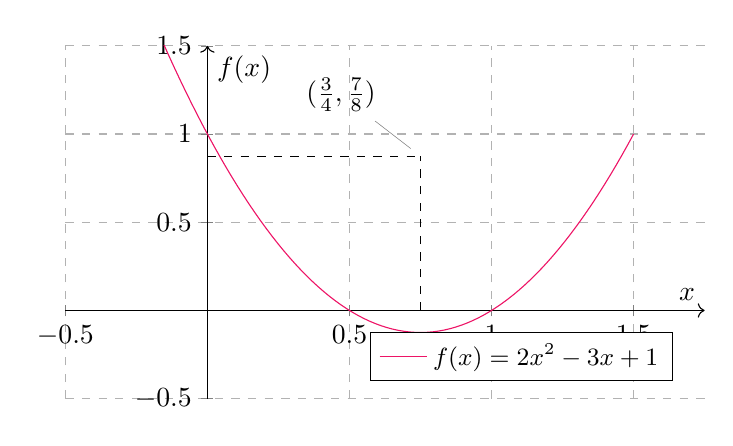
\begin{tikzpicture}
    \begin{axis}[
        xlabel=$x$,
        ylabel=$f(x)$,
        xmin=-0.5, xmax=1.75,
        ymin=-0.5, ymax=1.5,
        axis lines=middle,
        axis line style={->},
        legend style={at={(0.95,0.05)},anchor=south east},
        grid=both,
        major grid style={dashed,gray!60},
        width=0.8\textwidth,
        height=0.5\textwidth,
        legend style={font=\small},
        legend cell align={left},
    ]
    \addplot[WildStrawberry,domain=-0.5:1.5, samples=100] {2*x^2 - 3*x + 1};
    \legend{$f(x) = 2x^2 - 3x + 1$}
    
    \node[pin=135:{$(\frac{3}{4}, \frac{7}{8})$}] at (axis cs:0.75,0.875) {};
    \draw[dashed] (axis cs:0.75,0) -- (axis cs:0.75,0.875);
    \draw[dashed] (axis cs:0,0.875) -- (axis cs:0.75,0.875);
    
    \end{axis}
\end{tikzpicture}
\end{center}

\subsection*{\hl{Remember!}}

\begin{minipage}{\textwidth}
\textbf{Parabolas (Standard Form)}

\begin{tabularx}{\textwidth}{|X|X|}
\hline
\textbf{Equation} & $y = ax^2 + bx + c$ \\
\hline
\textbf{Vertex} & $(-\frac{b}{2a}, -\frac{b^2-4ac}{4a})$ \\
\hline
\textbf{Opening Direction} & Down if $a > 0$ \\
\hline
\textbf{Y-intercept} & $(0, c)$ \\
\hline
\end{tabularx}

\textbf{Parabolas (Vertex Form)}

\begin{tabularx}{\textwidth}{|X|X|}
\hline
\textbf{Equation} & $y = a(x - h)^2 + k$ \\
\hline
\textbf{Vertex} & $(h, k)$ \\
\hline
\textbf{Opening Direction} & Up if $a > 0$, Down if $a < 0$ \\
\hline
\end{tabularx}
\end{minipage}

\newpage
\subsection{Applications of Quadratic Functions}

Quadratic functions are not merely theoretical; they have numerous practical applications in various fields. Some common applications include:

\begin{enumerate}
    \item \textbf{Physics}: Quadratic functions describe the motion of objects under the influence of gravity. The equation $h(t) = -16t^2 + v_0t + h_0$ models the height ($h$) of an object at time ($t$) when it is thrown vertically with an initial velocity ($v_0$) from an initial height ($h_0$).

    \item \textbf{Engineering}: In structural engineering, quadratic equations model the deformation of materials under load, helping engineers design stable structures.

    \item \textbf{Economics}: Quadratic functions are used to model cost, revenue, and profit functions in business and economics. These functions assist in optimizing production and pricing strategies.

    \item \textbf{Computer Graphics}: In computer graphics, quadratic functions are used to create smooth curves and surfaces. For instance, Bézier curves are defined using quadratic equations.

    \item \textbf{Biology}: Quadratic functions can model population growth or decline of species. The logistic growth model is an example of such an application.

    \item \textbf{Statistics}: In regression analysis, quadratic functions are used to model complex relationships between variables.

    \item \textbf{Astronomy}: Quadratic equations can describe the orbits of celestial bodies and the motion of planets.

\end{enumerate}
\begin{note}
Quadratic functions are versatile and play a fundamental role in mathematics and various scientific disciplines. Understanding their properties, equations, and applications is crucial to problem solving and modeling real-world phenomena. Whether in physics, engineering, economics, or any other field, the knowledge of quadratic functions is a valuable asset in tackling complex problems.
\end{note}

\section{Unit 4: Exponential Functions}
 
\subsection{Radicals}
\begin{lesson}{Parts of radicals}

$$\sqrt[n]{a}$$    
\begin{itemize}
\item \textcolor{blue}{n = index or root}
\item \textcolor{blue}{a = Radicand}
\end{itemize}
\end{lesson}

\begin{lesson}{PROPERTIES OF RADICALS }
\begin{enumerate}[label=\alph*.]
    \item $a^{\frac{1}{n}}=\sqrt[n]{a}$
    \item $a^{\frac{m}{n}}=\sqrt[n]{a}=(\sqrt[n]{a})^m$
    \item $\sqrt[n]{a^n} = a^{\frac{n}{n}}$
    \item $\sqrt[n]{ab} \cdot \sqrt[n]{b}$
\end{enumerate}
\end{lesson}

\begin{example}
\begin{enumerate}
    \item $x^{\frac{1}{3}} = \sqrt[3]{x}$ 
    \item $x^{\frac{2}{3}}= \sqrt[3]{x^2}$ or $(\sqrt[3]{x})^2$
    \item $\sqrt{x^2} = x$ \quad $\sqrt[5]{x^5}=x$
\end{enumerate}    
\end{example}
\newpage
\begin{example}
\begin{enumerate}
    \item $\sqrt{36y^4} = \sqrt{36} \cdot \sqrt{y^4}=6y^2$
    \item 2. $\sqrt{72y^5}= \sqrt{36y^4} \cdot \sqrt{2y}= 6y^2 \sqrt{2y}$
    \item $\sqrt[3]{48y^7}= \sqrt[3]{8y^6} \cdot \sqrt[3]{6y}=2y^2 \sqrt[3]{6y}$
    \item $\sqrt[4]{64x^5 y^8}= \sqrt[4]{16x^4y^8} \sqrt[4]{4x}=2xy^2 \sqrt[4]{4x}$
    \item $\sqrt[5]{64x^5y^8} = \sqrt[5]{32x^5y^5} \cdot \sqrt[5]{2y^5}=2xy^5 \sqrt{2y^5}$
    \item $\sqrt{\frac{9}{16}}= \frac{\sqrt{9}}{\sqrt{16}} =\frac{3}{4}$
    \item 7. $\sqrt[3]{\frac{8y^4}{27x^3}}=\frac{\sqrt[3]{8y^4}}{\sqrt[3]{27x^3}}=\frac{\sqrt[3]{8y^3} \cdot \sqrt[3]{y}}{\sqrt[3]{27x^3}}= \frac{2y^3 \sqrt{y}}{3x}$
    \item $\sqrt{\frac{x^2}{4y^2}}= \frac{\sqrt{x^2}}{\sqrt{4y^2}}= \frac{x}{2y}$
\end{enumerate}
\end{example}
\newpage
\begin{lesson}{Rationalizing the Denominator}
When simplifying fractions with radicals, you need to rationalize the denominator by multiplying the numerator and the denominator by the \textbf{smallest value that will allow you to eliminate the the radical in the denominator}, as shown below. 
\end{lesson}
\begin{example}
\begin{enumerate}
    \item $\sqrt{\frac{1}{5}}= \frac{\sqrt{1}}{\sqrt{5}}= \frac{1}{\sqrt{5}}\cdot \textcolor{red}{\frac{\sqrt{5}}{\sqrt{5}}}=\frac{\sqrt{5}}{\sqrt{25}}=\frac{\sqrt{5}}{5}$
    \item $\sqrt{\frac{2}{3}}= \frac{\sqrt{2}}{\sqrt{3}} \cdot \textcolor{red}{\frac{\sqrt{3}}{\sqrt{3}}} = \frac{\sqrt{6}}{3}$ 
    \item $\sqrt[3]{\frac{1}{x}} = \frac{\sqrt[3]{1}}{\sqrt[3]{x}}= \frac{1}{\sqrt[3]{x}} \cdot \textcolor{red}{\frac{\sqrt[3]{x^2}}{\sqrt[3]{x^2}}}= \frac{\sqrt[3]{x^2}}{\sqrt[3]{x^3}}= \frac{\sqrt[3]{x^2}}{x}$
    \item $\sqrt[4]{\frac{4p^8}{8p^8}}= \sqrt[4]{\frac{p^2}{2}}= \frac{\sqrt[4]{p^2}}{\sqrt[4]{2}} \cdot \textcolor{red}{\frac{\sqrt[4]{2^3}}{\sqrt[4]{2^3}}}=\frac{\sqrt[4]{8p^2}}{2}$
\end{enumerate}    
\end{example}
\begin{note}
Rules for Simplifying Radicals:
\begin{enumerate}
\item There should be no factor in the radicand that has a power greater than or equal to the index.
\item There should be no fractions under the radical sign.
\item There should be no radicals in the denominator (i.e. the denominator should be rationalized).
\end{enumerate}
\end{note}
\newpage 
\begin{lesson}{ADDITION AND SUBTRACTION}

    Radicals may be added or subtracted when they have the same index \underline{and} the same radicand(just like combining like terms).
\begin{note}
    When adding or subtracting radicals, the index and radicand do \underline{not} change.
\end{note}    
\end{lesson}
\begin{example}
\begin{enumerate}
    \item $5\sqrt{2}-8\sqrt{2}=-3\sqrt{2}$
    \item $6x\sqrt[3]{3}+2x\sqrt[3]{3}= 8x\sqrt[3]{3}$
    \item $5\sqrt[5]{xy}+6\sqrt[5]{xy}= 11\sqrt[5]{xy}$
    \item $7\sqrt{x} - 9\sqrt[3]{x} +4\sqrt[3]{x}= 7 \sqrt{x} - 5\sqrt[3]{x}$
    \item $\sqrt{75}+2\sqrt{12}-5\sqrt{3}=\sqrt{25}\sqrt{3}+2\sqrt{4}\sqrt{3}-5\sqrt{3}+4\sqrt{3}-5\sqrt{5}=4\sqrt{3}$
\end{enumerate}    
\end{example}
\newpage
\begin{lesson}{MULTIPLICATION OF RADICALS}
    To multiple radicals, just multiply using the same rules as multiplying polynomials (Distributive Property, FOIL, and Exponent Rules) except \textbf{NEVER} multiply values outside of the radicals times values inside the radical.
\end{lesson}
\begin{example}
\begin{enumerate}
    \item $\sqrt{20x^3} \cdot \sqrt{4xy^6}= \sqrt{80x^4y^7}=\sqrt{16x^4y^6} \cdot \sqrt{5y} = 4x^2y^3\sqrt{5y}$
    \item $2x\sqrt{3xy} \cdot 4\sqrt{2x^5y}$
    \item $2\sqrt{5}(3\sqrt{2}-\sqrt{5})=6\sqrt{10}-2\sqrt{25}=  6\sqrt{10}-10$
    \item $(2\sqrt{x}+2)(\sqrt{x}+3)=2\sqrt{x^2}+6\sqrt{x}+2\sqrt{x}+6$
\end{enumerate}    
\end{example}
\begin{note}
When multiplying radicals with different indexes, change to rational exponents first, find a common denominator in order to add the exponents, then rewrite in radical notation as shown below: \\
Example: $\sqrt[3]{x^2} \cdot \sqrt[6]{x^5}=x^{\frac{2}{3}} \cdot x^{\frac{5}{6}}= x^{\frac{4}{6}}\cdot x^{\frac{5}{6}}= x^{\frac{3}{2}}=\sqrt{x^3}=\sqrt{x^2}\sqrt{x}=x\sqrt{x}$
\end{note}
\newpage
\begin{lesson}{MORE RATIONALIZING THE DENOMINATOR: (DIVISION)}
    If the denominator contain two terms such that at least one term has a radical, multiply the numerator and the denominator by the \textbf{conjugate} of the denominator:
    \textbf{Conjugate} - the conjugate of a binomial of the form (a+b) is (a-b).
    Example: The conjugate of $(\sqrt{x}-3) is (\sqrt{x}+3).$
\end{lesson}
\begin{note}
    Since $(a+b)(a-b)=a^2-b^2$, eliminating the middle term, multiplying by the conjugate eliminates the middle term that would still have a radical in it, thus removing the radical from the denominator.
\end{note}
\begin{example}
\begin{align*}
    &a. \frac{1}{\sqrt{x}+1} \cdot \frac{\sqrt{x}-1}{\sqrt{x}-1} = \frac{\sqrt{x}-1}{\sqrt{x^2}-1} = \frac{\sqrt{x}-1}{x-1} \\
    &b. \frac{6}{\sqrt{5}-\sqrt{2}} \cdot \frac{\sqrt{5}+\sqrt{2}}{\sqrt{5}+\sqrt{2}} = \frac{6(\sqrt{5}+\sqrt{2})}{5-2} = \frac{6(\sqrt{5}+\sqrt{2})}{3} = 2(\sqrt{5}+\sqrt{2})
\end{align*}
\end{example}
\newpage
\subsection{Exponent Laws}
\begin{lesson}{Exponent Laws}
 
\subsection*{Product Law}
When multiplying two terms with the same base, add the exponents.
\[ a^m \cdot a^n = a^{m + n} \]

\subsection*{Quotient Law}
When dividing two terms with the same base, subtract the exponents.
\[ \frac{a^m}{a^n} = a^{m - n} \]

\subsection*{Power Law}
When raising a power to another power, multiply the exponents.
\[ (a^m)^n = a^{mn} \]

\subsection*{Zero Exponent Law}
Any nonzero number raised to the power of zero is equal to 1.
\[ a^0 = 1 \]

\subsection*{Negative Exponent Law}
\[ a^{-n} = \frac{1}{a^n} \]
\subsection*{Exponent Laws}
\begin{enumerate}[label=\arabic*.]
    \item \( x^3 \cdot x^4 = x^{3 + 4} = x^7 \)
    \item \( \frac{y^6}{y^3} = y^{6 - 3} = y^3 \)
    \item \( a^5 \cdot a^{-2} = a^{5 - 2} = a^3 \)
    \item \( \frac{b^8}{b^4} = b^{8 - 4} = b^4 \)
\end{enumerate}
\newpage
\subsection{Logarithms}
\begin{lesson}{Logarithms}
\subsection*{Introduction to Logarithms}
Logarithms are the inverse operations of exponentiation.

\subsection*{Properties of Logarithms}
\begin{enumerate}[label=\alph*.]
    \item \( \log_b(a \cdot c) = \log_b(a) + \log_b(c) \)
    \item \( \log_b\left(\frac{a}{c}\right) = \log_b(a) - \log_b(c) \)
    \item \( \log_b(a^n) = n \cdot \log_b(a) \)
\end{enumerate}

\subsection*{Common Logarithm and Natural Logarithm}
\begin{enumerate}[label=\alph*.]
    \item Common logarithm: \( \log_{10}(x) = \log(x) \)
    \item Natural logarithm: \( \ln(x) \)
\end{enumerate}
\end{lesson}
\subsection*{Examples}
\subsection*{Logarithms}
\begin{enumerate}[label=\arabic*.]
    \item \( 10^x = 100 \) implies \( x = 2 \)
    \item \( \log_2(8) = 3 \) because \( 2^3 = 8 \)
    \item \( e^y = 20 \) implies \( y = \ln(20) \)
    \item \( \ln(1) = 0 \) because \( e^0 = 1 \)
\end{enumerate}
\end{lesson}
\newpage 
\begin{lesson}{Solving equations with logarithms}
\begin{arrowlist}
 \item The logarithms of a \# to given base is the exponent that must be used with that base to obtain the given \#.
 \begin{example}
     The logarithms of $64$ to base $2$ is $6$ since $2^6 = 64$
 \end{example}
 We would write that as: $\log_2 64 = 6$.
 \begin{itemize}
     \item $\log_2$ - base.
     \item $64$ - argument.
     \item $6$ - logarithms.
 \end{itemize}

\item The logarithm function is the $\underbrace{\textbf{\textcolor{blue}{inverse}}}_{\text{(Switch $x$ and $y$)}}$ function of an exponent.

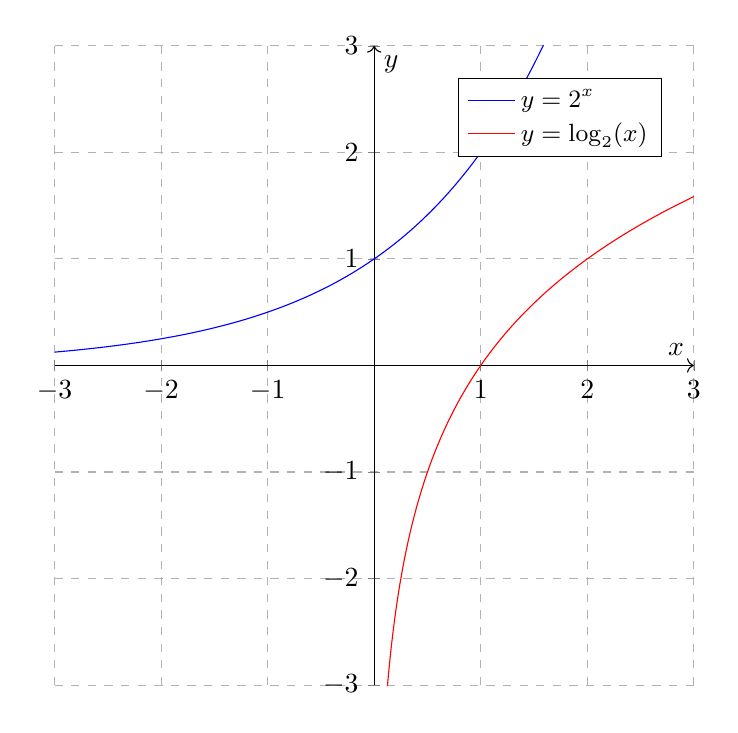
\begin{tikzpicture}
    \begin{axis}[
        xlabel=$x$,
        ylabel=$y$,
        xmin=-3, xmax=3,
        ymin=-3, ymax=3,
        axis lines=middle,
        axis line style={->},
        legend style={at={(0.95,0.95)},anchor=north east},
        grid=both,
        major grid style={dashed,gray!60},
        width=0.8\textwidth,
        height=0.8\textwidth,
        legend style={font=\small},
        legend cell align={left},
    ]
    
    % Plot y=2^x
    \addplot[blue, domain=-3:2, samples=100, smooth] {2^x};
    \addlegendentry{$y = 2^x$}
    
    % Plot y=log_2(x)
    \addplot[red, domain=0.1:3, samples=100, smooth] {log2(x)};
    \addlegendentry{$y = \log_2(x)$}
    
    \end{axis}
\end{tikzpicture}
\end{arrowlist}

\newpage
\begin{arrowlist}
 \item In general we write $y= \log_a x$ where a is the base and x is the argument 
\end{arrowlist}
\end{lesson}
\begin{example}
Determine the logs:
\begin{enumerate}[label=\alph*.]
    \item $\log_{10} 1000= 3$ since $10^3=1000$
    \item $\log_5 625 = 5^x= 625= x=4$
    \item $\log_2 1024= 10$
    \item $\log_b b=1$
    \item $\log_2 1=0$
\end{enumerate}
\end{example}
\begin{example}
Express in exponential form:
    \begin{enumerate}
        \item $m =\log_3 81 \Rightarrow3^m=81$
        \item $y=\log_7 (\frac{1}{7}) \Rightarrow 7^y=\frac{1}{7}$
        \item $n=\log _a n \Rightarrow a^m=n$
    \end{enumerate}
\end{example}
\begin{example}
    Express as logarithm
    \begin{enumerate}
        \item $2^5=32 \Rightarrow 5=\log_2 32$
        \item $3^m=343 \Rightarrow m=\log_3 343$
        \item $\frac{1}{25}= 5^x \Rightarrow n=\log_5 (\frac{1}{25})$
    \end{enumerate}
\end{example}
\newpage
\begin{example}
Use your calculator to Evaluate
    \begin{enumerate}
        \item $\log_6 216 \Rightarrow 3$
        \item $\log_7 117649 \Rightarrow \frac{\log 117649}{\log 7}=6$
        \item $\log 1000000 \Rightarrow$ base 10(common log) $=6$
    \end{enumerate}
\end{example}

\begin{empheq}[box = {\Garybox[Log law]}]{align*}
    1. & \log a^x \Rightarrow x \log a \\
    2. & a^x = (10^{\log a})^x \Rightarrow a^x =10^{x \log a}
\end{empheq}
\begin{example}
    \begin{enumerate}
        \item $12^x=400 \Rightarrow x = \log_12 400= x=\frac{\log 400}{log 12}= x \approx 2.41$
        \item $1.08^x=4.39 \Rightarrow \log 10.8^x = \log 4.39= x=\frac{log 4.39}{1.08}=x \approx 19.22$
        \item $10^{x-3}=500$
        \begin{align*}
        10^{x-3} &= 500 \\
        \Rightarrow \log 10^{x-3} &= \log 500 \\
        (x-3) \log 10 &= \log 500 \\
        x-3 &= \frac{\log 500}{\log 10} \\
        x-3 &= \frac{\log 500}{\log 10} \\
        x &= 3 + \frac{\log 500}{\log 10} \\
        x &\approx 5.70
    \end{align*}
    \end{enumerate}
\end{example}
\newpage
\subsection{Transformation of Exponential Function}
\begin{equation*}
    \underbrace{f(x)=a \cdot b ^{k(k-d)}+C}_{\text{base of exponential f\underline{n}}}
\end{equation*}
Exponential functions can be transformed in the same way as $f(x)=a \cdot b ^{k(k-d)}+C$
other function. The graph of can be found by
performing transformations on the graph of y = bx
\begin{example}
    List transformation applied to \(y=2^x\)
    \begin{enumerate}
        \item \(f(x)=3 \cdot 2^x-5\)
        \begin{itemize}
            \item \textcolor{red}{VS by 3}
            \item \textcolor{red}{Parent function \(y=2^x\)}
            \item \textcolor{red}{VT 5 \(\downarrow\)}
        \end{itemize}
        \item \(f(x)=-2^{x-1}+6\)
        \begin{itemize}
            \item \textcolor{red}{RXA}
            \item \textcolor{red}{HT 1 \(\to\)}
            \item \textcolor{red}{VT 6 \(\uparrow\)}
        \end{itemize}
        \item \(f(x)=\frac{1}{2}(2)^{-x+4} -8\)
        \begin{itemize}
            \item \textcolor{red}{VS by 2}
            \item \textcolor{red}{RXA}
            \item \textcolor{red}{HT 4 \(\to\)}
            \item \textcolor{red}{VT 6 \(\uparrow\)}
        \end{itemize}
        \item \(f(x)=-2^{3x-9}+62\)
        \begin{itemize}
            \item \textcolor{red}{RXA}
            \item \textcolor{red}{HS by \(\frac{1}{3}\)}
            \item \textcolor{red}{VT 62 \(\uparrow\)}
        \end{itemize} 
    \end{enumerate}
\end{example}
\newpage
\begin{example}
    List the the transformation applied to \(y=\left(\frac{1}{4}\right)^x\)
    \begin{enumerate}
        \item $f(x)=3 \left( \frac{1}{4}\right)^{x-10}-8$
    \begin{itemize}
    \item \textcolor{red}{VS}
    \item \textcolor{red}{HT 10 \(\to\)}
    \item \textcolor{red}{VT 8 \(\downarrow\)}
    \end{itemize}  
    \item $g(x)=-\left(\frac{1}{4} \right)^{\frac{1}{2}x}+2$
    \begin{itemize}
    \item \textcolor{red}{RXA}
    \item \textcolor{red}{HS by \(2\)}
    \item \textcolor{red}{VT 2 \(\downarrow\)}
    \end{itemize}     
    \item $h(x)=\frac{1}{3}\left(\frac{1}{4}\right)^{-x-6}$
    \begin{itemize}
    \item \textcolor{red}{VS by \(\frac{1}{3}\)}
    \item \textcolor{red}{RYA}
    \item \textcolor{red}{HT 6 \(\gets\)}
    \end{itemize}       
    \item $p(x)=-3\left( \frac{1}{4}\right)^{2x+1}$
    \begin{itemize}
    \item \textcolor{red}{RXA}
    \item \textcolor{red}{VS by 3}
    \item \textcolor{red}{HT by \(\frac{1}{2}\)}
    \item \textcolor{red}{HS by \(\frac{1}{2}\)}
    \end{itemize}    
    \end{enumerate}
\end{example}
\newpage 
For an exponential function, the horizontal asymptote is only affected by vertical translation. So the equation of the H.A will be $y=c$ \\ \\
When the function is: \\ 
\begin{equation*}
f(x)=a\cdot b^{k(x-d)}+C    
\end{equation*}
\begin{example}
    Find the equation of the horizontal asymptote and determine the $y$-intercept (set $x = 0$).
    \begin{enumerate}
        \item $f(x)=2\cdot 3^x -4 \quad $ H.A $= -4 \quad$ y-int is -2
        \item $g(x)=\frac{1}{2}\left(\frac{1}{8} \right)^{-x}+1 \quad $ H.A $=1 \quad$  y-int is $\frac{3}{2}$
    \end{enumerate}
\end{example}
\begin{lesson}{Exponential Functions}
    \begin{arrowlist}
        \item The domain of exponential function is always: $\{x \in \mathbb{R}\}$. 

        \begin{figure}[h]
            \centering
            \begin{subfigure}{0.45\textwidth}
                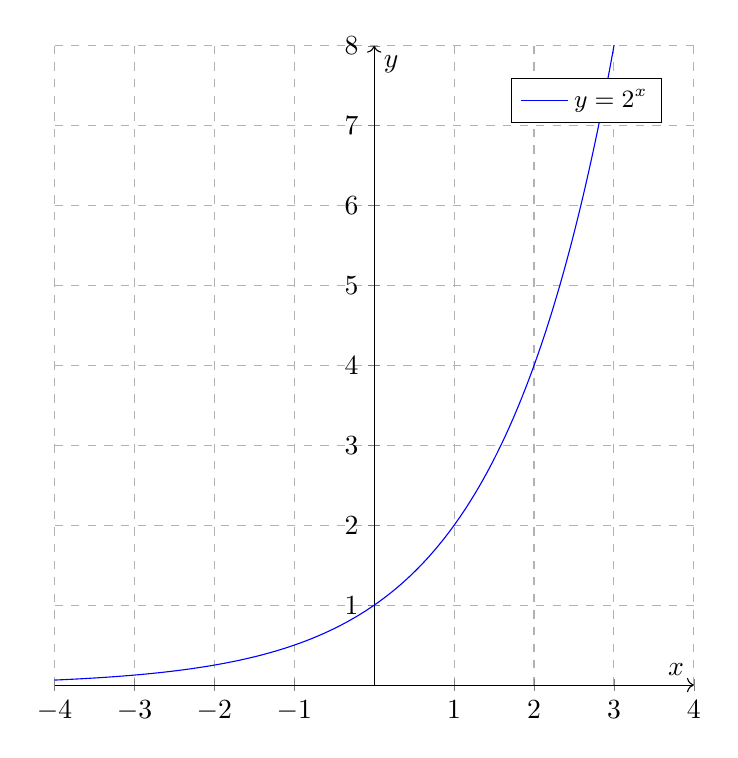
\begin{tikzpicture}
                    \begin{axis}[
                        xlabel=$x$,
                        ylabel=$y$,
                        xmin=-4, xmax=4,
                        ymin=0, ymax=8,
                        axis lines=middle,
                        axis line style={->},
                        legend style={at={(0.95,0.95)},anchor=north east},
                        grid=both,
                        major grid style={dashed,gray!60},
                        width=0.8\textwidth,
                        height=0.8\textwidth,
                        legend style={font=\small},
                        legend cell align={left},
                    ]

                    % Growth function
                    \addplot[blue, domain=-4:4, samples=100, smooth] {2^x};
                    \addlegendentry{$y = 2^x$}

                    \end{axis}
                \end{tikzpicture}
                \caption{Growth}
                \label{fig:growth}
            \end{subfigure}
            %
            \begin{subfigure}{0.45\textwidth}
                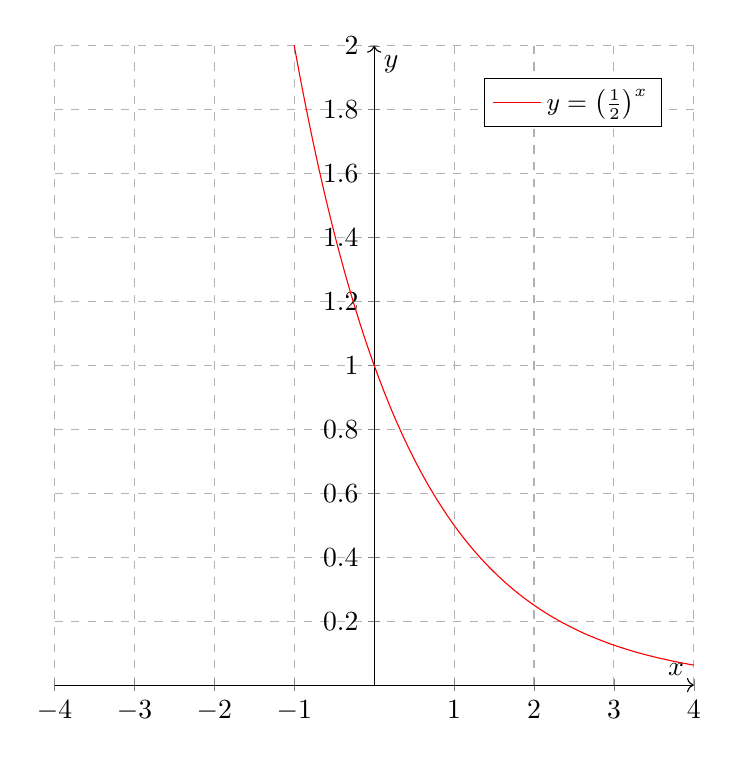
\begin{tikzpicture}
                    \begin{axis}[
                        xlabel=$x$,
                        ylabel=$y$,
                        xmin=-4, xmax=4,
                        ymin=0, ymax=2,
                        axis lines=middle,
                        axis line style={->},
                        legend style={at={(0.95,0.95)},anchor=north east},
                        grid=both,
                        major grid style={dashed,gray!60},
                        width=0.8\textwidth,
                        height=0.8\textwidth,
                        legend style={font=\small},
                        legend cell align={left},
                    ]

                    % Decay function
                    \addplot[red, domain=-4:4, samples=100, smooth] {(1/2)^x};
                    \addlegendentry{$y = \left(\frac{1}{2}\right)^x$}

                    \end{axis}
                \end{tikzpicture}
                \caption{Decay}
                \label{fig:decay}
            \end{subfigure}

            \caption{Growth and Decay}
            \label{fig:growth_decay}
        \end{figure}

        \item The range will depend on the location of the horizontal asymptote and if there was a reflection in the x-axis (RXA).
    \end{arrowlist}
    
% Growth and Decay in 3D plot     
\begin{figure}[H]
    \centering
    \begin{tikzpicture}
        \begin{axis}[
            xlabel=$x$,
            ylabel=$y$,
            zlabel=$z$,
            xmin=-4, xmax=4,
            ymin=0, ymax=8,
            zmin=0, zmax=8,
            axis lines=middle,
            axis line style={->},
            legend style={at={(0.95,0.95)},anchor=north east},
            grid=both,
            major grid style={dashed,gray!60},
            width=0.8\textwidth,
            height=0.8\textwidth,
            legend style={font=\small},
            legend cell align={left},
            view={40}{30}, % Adjust the view angle
            colormap/jet, % Use 'hot' colormap
        ]
            \addplot3[surf,hot,domain=-4:4,domain y=0:8,shader=interp] {2^x};
            \addlegendentry{$z = 2^x$}
        \end{axis}
    \end{tikzpicture}
    \qquad
    \begin{tikzpicture}
        \begin{axis}[
            xlabel=$x$,
            ylabel=$y$,
            zlabel=$z$,
            xmin=-4, xmax=4,
            ymin=0, ymax=8,
            zmin=0, zmax=8,
            axis lines=middle,
            axis line style={->},
            legend style={at={(0.95,0.95)},anchor=north east},
            grid=both,
            major grid style={dashed,gray!60},
            width=0.8\textwidth,
            height=0.8\textwidth,
            legend style={font=\small},
            legend cell align={left},
            view={40}{30}, % Adjust the view angle
            colormap/hot, % Use 'hot' colormap
        ]
            \addplot3[surf,hot,domain=-4:4,domain y=0:8,shader=interp] {(1/2)^x};
            \addlegendentry{$z = \left(\frac{1}{2}\right)^x$}
        \end{axis}
    \end{tikzpicture}
    \caption{Growth and Decay in 3D Plot}
\end{figure}
\end{lesson}
\newpage 


\newpage
\subsection*{Examples}
\begin{example}
\begin{enumerate}
   \item $f(x) = 2^x + 4$
   
   \begin{minipage}{0.8\textwidth}
       \begin{tikzpicture}
            \begin{axis}[
                xlabel=$x$,
                ylabel=$f(x)$,
                xmin=-2, xmax=2,
                ymin=2, ymax=8,
                axis lines=middle,
                axis line style={->},
                legend style={at={(0.95,0.95)},anchor=north east},
                grid=both,
                major grid style={dashed,gray!60},
                width=\textwidth,
                height=0.6\textwidth,
                legend style={font=\small},
                legend cell align={left},
            ]

            % Function
            \addplot[blue, domain=-2:2, samples=100, smooth] {2^x + 4};

            % Asymptote
            \draw[dashed, red] (axis cs:-2,4) -- (axis cs:2,4) node[midway,above left,red]{$y=4$};

            \end{axis}
        \end{tikzpicture}
   \end{minipage}
   \vspace{0.5cm}
   
   $\{y \in \mathbb{R} \mid y > 4\}$    
   
    \item $g(x) = -2^x + 2$

    
    \begin{minipage}{0.8\textwidth}
        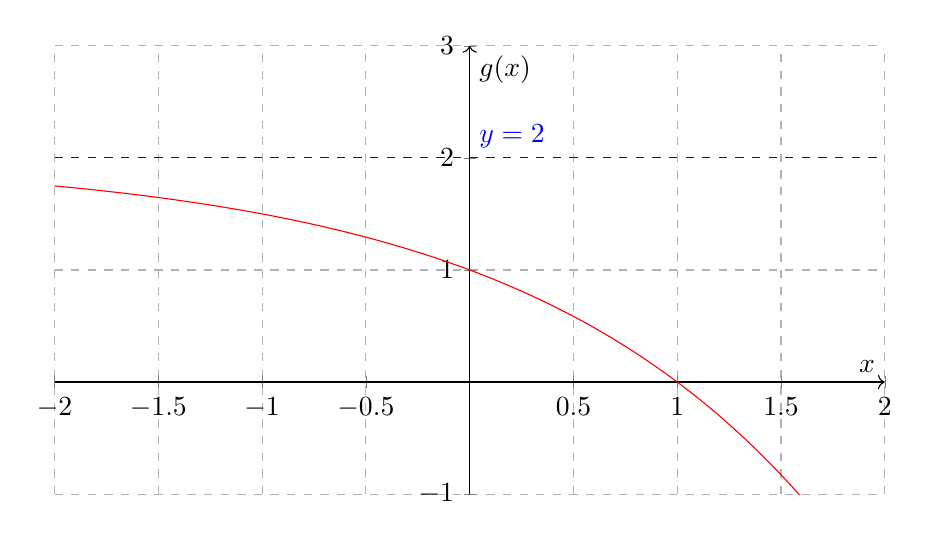
\begin{tikzpicture}
            \begin{axis}[
                xlabel=$x$,
                ylabel=$g(x)$,
                xmin=-2, xmax=2,
                ymin=-1, ymax=3,
                axis lines=middle,
                axis line style={->},
                legend style={at={(0.95,0.95)},anchor=north east},
                grid=both,
                major grid style={dashed,gray!60},
                width=\textwidth,
                height=0.6\textwidth,
                legend style={font=\small},
                legend cell align={left},
            ]

            % Function
            \addplot[red, domain=-2:2, samples=100, smooth] {-2^x + 2};

            % Asymptote
            \draw[dashed, blue] (axis cs:-2,2) -- (axis cs:2,2) node[midway,above right,blue]{$y=2$};

            \end{axis}
        \end{tikzpicture}
    \end{minipage}
   \vspace{0.5cm}
   
   $\{y \in \mathbb{R} \mid y < 2\}$   
\end{enumerate}
\end{example}

\newpage 
\begin{example}
    Ex.1: For the function, find:
        \begin{enumerate}
            \item Parent function 
            \item Horiz asymptote
            \item y-int
            \item Transformations
            \item Domain \& Range 
        \end{enumerate}
    \begin{enumerate}[label=\alph*.]
    \item $f(x)= 4^{2(x+5)}-8$ \\
    Parent function: $4^x$ \\
    Transformation: 
    \begin{enumerate}
        \item HS by $\frac{1}{2}$
        \item HT 5 $\gets$
        \item VT 8 $\downarrow$
    \end{enumerate}
    y-int:
    \begin{align*}
        f(0) & = 4^{2(0+5)}-8 \\
        & = 4^{10}-8 \\
        & = 1048568
    \end{align*}
    H.A: $ y= -8$ \\ 
    Domain: $\{x \in \mathbb{R}\}$
    Range:  $\{y \in \mathbb{R} \mid y > -8\}$
    \end{enumerate}
\end{example}

\newpage 
\begin{lesson}{Graphing Exponential Functions}
\underline{Ex.1}: The function \(y=3^x\) is an exponential function because the exponent is a variable.\\

Now, let's look at how to graph the exponential function \(y=3^x\).

\begin{table}[h]
    \centering
    \begin{minipage}{0.5\linewidth}
        \centering
    \begin{tabular}{|c|c|c|c|}
    \hline
    $x$ & $y=3^x$ & $y$ & $(x,y)$ \\
    \hline
    $-3$ & $3^{-3} = \frac{1}{3^3}$ & $\frac{1}{27}$ & $(-3, \frac{1}{27})$ \\
    $-2$ & $3^{-2} = \frac{1}{3^2}$ & $\frac{1}{9}$ & $(-2, \frac{1}{9})$ \\
    $-1$ & $3^{-1} = \frac{1}{3^1}$ & $\frac{1}{3}$ & $(-1, \frac{1}{3})$ \\
    $0$ & $3^0 = 1$ & $1$ & $(0, 1)$ \\
    $1$ & $3^1 = 3$ & $3$ & $(1, 3)$ \\
    $2$ & $3^2 = 9$ & $9$ & $(2, 9)$ \\
    $3$ & $3^3 = 27$ & $27$ & $(3, 27)$ \\
    \hline 
    \end{tabular}

    \end{minipage}%
    \begin{minipage}{0.5\linewidth}
        \centering
        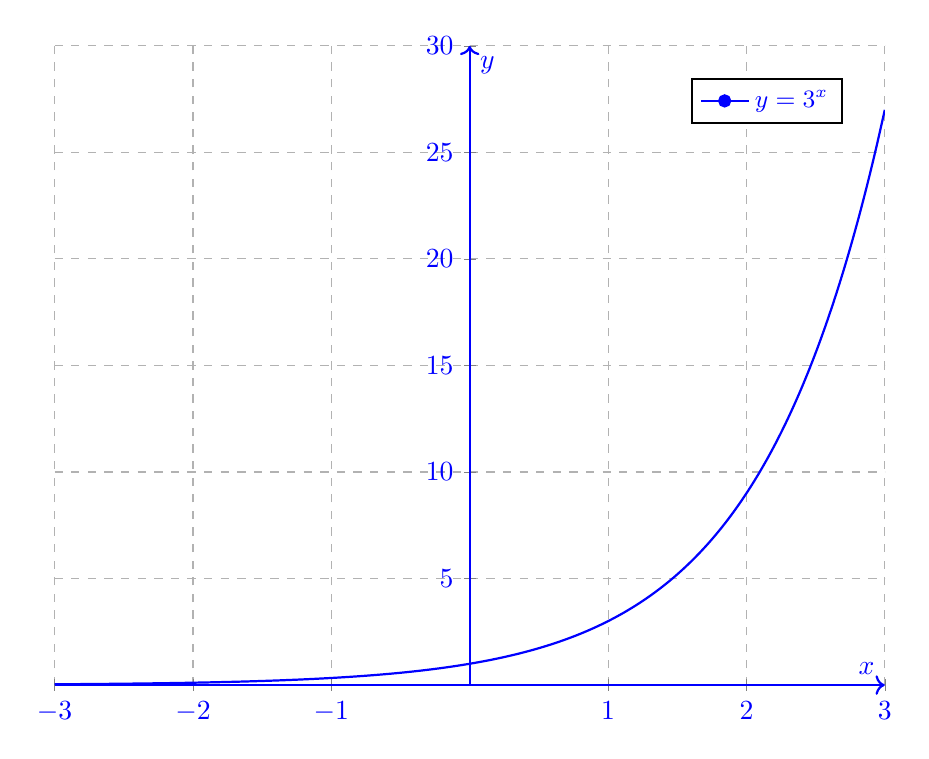
\begin{tikzpicture}
            \begin{axis}[
                xlabel=$x$,
                ylabel=$y$,
                xmin=-3, xmax=3,
                ymin=0, ymax=30,
                axis lines=middle,
                axis line style={->},
                legend style={at={(0.95,0.95)},anchor=north east},
                grid=both,
                major grid style={dashed,gray!60},
                width=\linewidth,
                height=0.8\textwidth,
                legend style={font=\small},
                legend cell align={left},
                domain=-3:3,
                samples=100,
                smooth,
                blue,
                thick,
                mark=*,
                mark options={blue,fill=blue}
            ]
            
            % Plot y=3^x
            \addplot[blue] {3^x};
            \addlegendentry{$y = 3^x$}
            
            \end{axis}
        \end{tikzpicture}
    \end{minipage}
\end{table}
\textbf{\underline{Definition 1}}: Since the y values increase as the x values increase in the example above, this is what we call exponential \textbf{\textcolor{blue}{Growth}}. (The graph goes up the hill from left to right) \\ \\
\textbf{\underline{QUESTION}}: In the exponential function \(y=3^x\), the y=values can never equal or be less than \textbf{\underline{zero}}. \\ \\ 

\textbf{\underline{Definition 2}}: Since the y-values can NEVER equal to zero in this function, there is a horizontal \underline{asymptote} at \(y=0\). \\ \\ 

\underline{\textbf{Ex.2}}: By looking at the graph above, list the domain and range of the function \(y=3^x\).\\

\textbf{Domain}:$\{x \in \mathbb{R}\}$. This is because the function is defined for every real value of \(x\). \\

\textbf{Range}: $\{y \in \mathbb{R} \mid y > 0\}$. This is evident from the graph, where the values of \(y\) are positive for all corresponding values of \(x\). \\ \\ 
\end{lesson}
\underline{\textbf{Ex.3}}: Consider the function \(y=\left(\frac{1}{3}\right)^x\). Analyze the graph and determine its domain and range.\\

\begin{table}[h]
    \centering
    \begin{minipage}{0.5\linewidth}
        \centering
        \begin{tabular}{|c|c|c|c|}
            \hline
            $x$ & $y=\left(\frac{1}{3}\right)^x$ & $y$ & $(x,y)$ \\
            \hline
            $-3$ & $27$ & $27$ & $(-3, 27)$ \\
            $-2$ & $9$ & $9$ & $(-2, 9)$ \\
            $-1$ & $3$ & $3$ & $(-1, 3)$ \\
            $0$ & $1$ & $1$ & $(0, 1)$ \\
            $1$ & $\frac{1}{3}$ & $\frac{1}{3}$ & $(1, \frac{1}{3})$ \\
            $2$ & $\frac{1}{9}$ & $\frac{1}{9}$ & $(2, \frac{1}{9})$ \\
            $3$ & $\frac{1}{27}$ & $\frac{1}{27}$ & $(3, \frac{1}{27})$ \\
            \hline 
        \end{tabular}
    \end{minipage}%
    \begin{minipage}{0.5\linewidth}
        \centering
        \begin{tikzpicture}
            \begin{axis}[
                xlabel=$x$,
                ylabel=$y$,
                xmin=-3, xmax=3,
                ymin=0, ymax=1,
                axis lines=middle,
                axis line style={->},
                legend style={at={(0.95,0.95)},anchor=north east},
                grid=both,
                major grid style={dashed,gray!60},
                width=\linewidth,
                height=0.8\textwidth,
                legend style={font=\small},
                legend cell align={left},
                domain=-3:3,
                samples=100,
                smooth,
                blue,
                thick,
                mark=*,
                mark options={blue,fill=blue}
            ]
            
            % Plot y=(1/3)^x
            \addplot[blue] {(1/3)^x};
            \addlegendentry{$y = \left(\frac{1}{3}\right)^x$}
            
            \end{axis}
        \end{tikzpicture}
    \end{minipage}
\end{table}
\textbf{\underline{Definition 2}}: Since the y-values decrease as the x-values increase in the example above, this is what we call exponential \textcolor{blue}{decay}. (The graph goes down the hill from left to right). \\ \\ 
\textbf{\underline{QUESTION}}: Is there an asymptote? If so, where it is? \\  \\
Yes , it is on "y=0".\\ \\
\underline{\textbf{Ex.4}}: By looking at the graph above, list the domain and range of the function \(y=(\frac{1}{3})^x\).\\ \\

\textbf{Domain}:$\{x \in \mathbb{R}\}$. This is because the function is defined for every real value of \(x\). \\

\textbf{Range}: $\{y \in \mathbb{R} \mid y > 0\}$. This is evident from the graph, where the values of \(y\) are positive for all corresponding values of \(x\). \\ \\ 
\underline{\textbf{Ex.3}}: Consider the function \(y=\left(\frac{1}{3}\right)^x\). Analyze the graph and determine its domain and range.\\
\begin{lesson}{1 - Exponential Growth}
\textcolor{blue}{Exponential growth} is a captivating concept where a quantity increases at a fixed percentage rate over time. This growth is modeled by the formula $y = ab^x$, where $a$ is the initial amount, $b$ is the growth factor, and $x$ is the time variable.

\begin{example}
Suppose you invest $1000$ at an annual interest rate of $5\%$, compounded annually. The growth formula is $A = 1000 \times (1 + 0.05)^x$. After 3 years, the amount would be approximately $A = 1000 \times (1 + 0.05)^3 \approx 1157.63$.
\end{example}

\begin{note}
The graph of an exponential growth function is characterized by a distinct upward curve that becomes steeper as $b$ increases.

\begin{center}
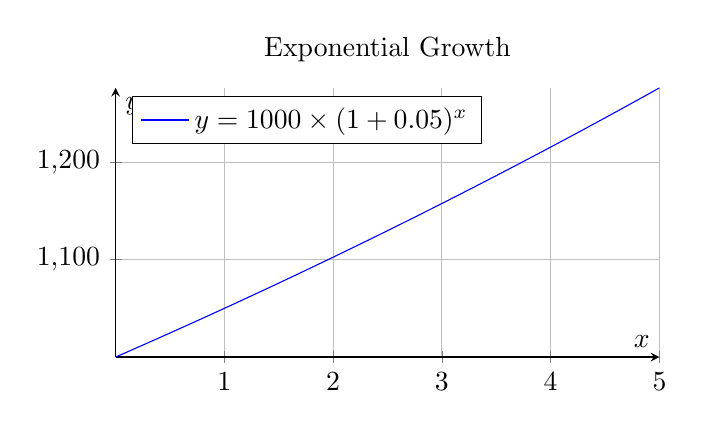
\begin{tikzpicture}
\begin{axis}[
  xlabel=$x$,
  ylabel=$y$,
  grid=major,
  axis lines=middle,
  width=0.7\linewidth,
  height=5cm,
  title={Exponential Growth},
  legend pos=north west,
]
\addplot[blue, domain=0:5, samples=100, smooth] {1000 * (1 + 0.05)^x};
\addlegendentry{$y = 1000 \times (1 + 0.05)^x$}
\end{axis}
\end{tikzpicture}
\end{center}
\end{note}
\end{lesson}
\newpage
\begin{lesson}{2 - Exponential Decay}
\textcolor{blue}{Exponential decay} is the counterpart to exponential growth. It occurs when a quantity decreases at a fixed percentage rate over time. The decay is modeled by the formula $y = ab^x$, where $b$ is between 0 and 1.

\begin{example}
Consider a radioactive substance that decays at a rate of 10\% per year. Its decay formula is $N = N_0 \times 0.9^t$. After 5 years, the remaining quantity is $N = N_0 \times 0.9^5$.
\end{example}

\begin{note}
The graph of an exponential decay function exhibits a decreasing curve that approaches but never reaches zero.

\begin{center}
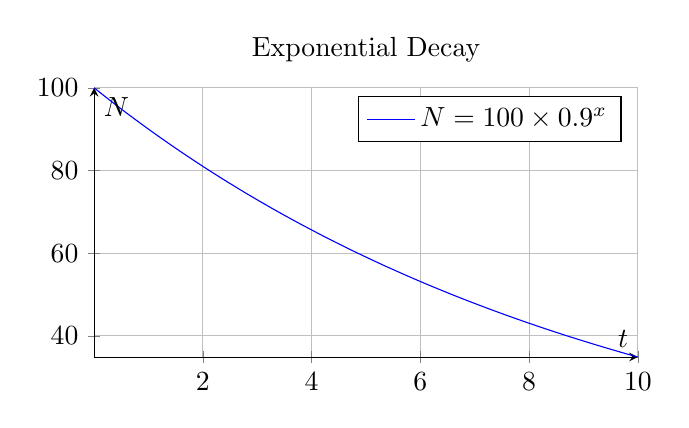
\begin{tikzpicture}
\begin{axis}[
  xlabel=$t$,
  ylabel=$N$,
  grid=major,
  axis lines=middle,
  width=0.7\linewidth,
  height=5cm,
  title={Exponential Decay},
  legend pos=north east,
]
\addplot[blue, domain=0:10, samples=100, smooth] {100 * 0.9^x};
\addlegendentry{$N = 100 \times 0.9^x$}
\end{axis}
\end{tikzpicture}
\end{center}
\end{note}
\end{lesson}
\newpage
\begin{lesson}{3 - Compound Interest}
\textcolor{blue}{Compound interest} is a powerful concept where interest is added to the initial principal, which then earns interest over time. The compound interest formula is given by $A = P(1 + r/n)^{nt}$, where $A$ is the final amount, $P$ is the principal, $r$ is the annual interest rate, $n$ is the number of times interest is compounded per year, and $t$ is the time in years.

\begin{example}
Imagine investing $5000$ at an annual interest rate of $6\%$, compounded quarterly. The formula is $A = 5000 \times (1 + 0.06/4)^{4t}$. After 2 years, the amount is $A = 5000 \times (1 + 0.06/4)^{4 \times 2}$.
\end{example}

\begin{note}
Compound interest enables your investment to grow faster compared to simple interest, especially with more frequent compounding.
\end{note}
\end{lesson}
\newpage 
\begin{lesson}{4 - Properties of Exponential Functions}
\textcolor{blue}{Exponential functions} possess several key properties:

\begin{itemize}
    \item They have a constant base.
    \item They can model growth or decay.
    \item They have an asymptote, which they approach but never reach.
    \item They are always positive if the base is greater than 1.
    \item They are always decreasing if the base is between 0 and 1.
\end{itemize}

\begin{example}
Consider the function $f(x) = 2^x$. It has a constant base of 2 and models exponential growth.
\end{example}

\begin{note}
The graph of an exponential function approaches but never crosses the horizontal axis (asymptote).

\begin{center}
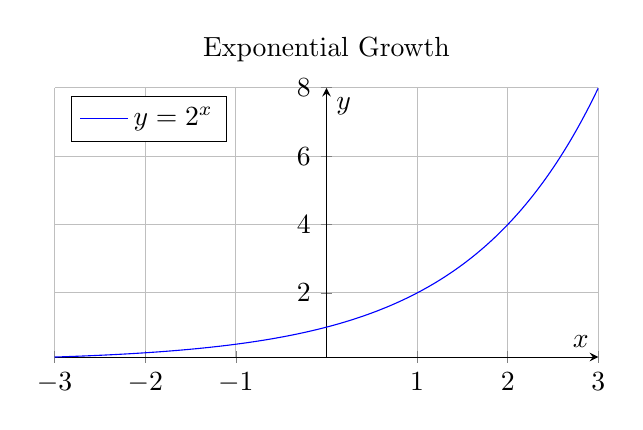
\begin{tikzpicture}
\begin{axis}[
  xlabel=$x$,
  ylabel=$y$,
  grid=major,
  axis lines=middle,
  width=0.7\linewidth,
  height=5cm,
  title={Exponential Growth},
  legend pos=north west,
]
\addplot[blue, domain=-3:3, samples=100, smooth] {2^x};
\addlegendentry{$y = 2^x$}
\end{axis}
\end{tikzpicture}
\end{center}
\end{note}
\end{lesson}
\newpage 
\begin{lesson}{5 - Transformations}
\textcolor{blue}{Transformations} offer a way to modify the graph of an exponential function. Common transformations include vertical shifts, horizontal shifts, reflections, and stretches or compressions. These transformations are applied to the base function $y = b^x$.

\begin{example}
If $g(x) = 3 \times 2^x$, the function $g$ is a vertical stretch of $f(x) = 2^x$ by a factor of 3.
\end{example}

\begin{note}
Transformations alter the appearance and behavior of the exponential function graph.

\begin{center}
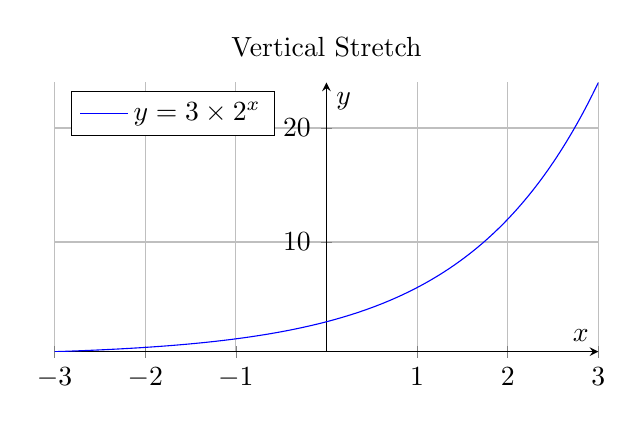
\begin{tikzpicture}
\begin{axis}[
  xlabel=$x$,
  ylabel=$y$,
  grid=major,
  axis lines=middle,
  width=0.7\linewidth,
  height=5cm,
  title={Vertical Stretch},
  legend pos=north west,
]
\addplot[blue, domain=-3:3, samples=100, smooth] {3 * 2^x};
\addlegendentry{$y = 3 \times 2^x$}
\end{axis}
\end{tikzpicture}
\end{center}
Transformations can also involve horizontal shifts, reflections, and other modifications to customize the behavior of the exponential function graph.
\end{note}
\end{lesson}



\newpage
\begin{lesson}{6 - Applications of Exponential Functions}
\begin{center}
\begin{minipage}{0.4\textwidth}
\begin{equation*}
    A = P(1+i)^n
\end{equation*}
\end{minipage}%
\begin{minipage}{0.6\textwidth}
Where:
\begin{itemize}
    \item A is the final amount
    \item P is the initial amount 
    \item i is the growth/decay rate
    \item n is the total number of growth/decay periods
\end{itemize}
\end{minipage}
\end{center}
Doubling Times: An increase of 100\% (or 1) which makes the base equal to 2. \\ \\
$$A = P(1+i)^n$$ 
$$\therefore A = P(2)^n$$
Half-Lives: A decrease of 50\%(or 0.5) which makes the base equal to $\frac{1}{2}$.
$$A=P(1-0.5)^n$$
$$\therefore A = P(0.5)$$
or
$$A = P(\frac{1}{2})^n$$
\end{lesson}
\begin{example}
    1.The element Duzzanium has a half-life of 4 months. If there are 5000 g of Duzzanium today, how much will there be in 2 years?
\end{example}
\begin{example}
    2. A bacterial culture began with 7500 bacteria. It's growth can be modeled using the formula $N=7500(2)^{\frac{t}{36}}$, where N is the number of bacteria after t hours.
\begin{enumerate}[label=\alph*.]
    \item What is the doubling time of the bacteria?
    \item How many bacteria are present after 36 hours?
    \item How many bacteria are present after 3 days?
    \item Approximately how many hours will pass for the culture to reach 2 million bacteria?
\end{enumerate}
    
\end{example}
\newpage

\newpage
\begin{lesson}{ Summative Assessment }
\begin{enumerate}
    \item \textbf{Evaluate the following:}
    \begin{enumerate}[label=\alph*)]
        \item $2^3$:
        \begin{align*}
            2^3 &= 2 \times 2 \times 2 \\
            &= 8
        \end{align*}
        
        \item $10^{-2}$:
        \begin{align*}
            10^{-2} &= \frac{1}{10^2} \\
            &= \frac{1}{100} \\
            &= 0.01
        \end{align*}
        
        \item $e^0$:
        \begin{align*}
            e^0 &= 1
        \end{align*}
    \end{enumerate}
    
    \item \textbf{Solve for $x$:}
    \begin{enumerate}[label=\alph*)]
        \item $5^x = 125$:
        \begin{align*}
            5^x &= 125 \\
            x &= 3
        \end{align*}
        
        \item $2e^{2x} = 16$:
        \begin{align*}
            e^{2x} &= 8 \\
            2x &= \ln(8) \\
            x &= \frac{\ln(8)}{2}
        \end{align*}
    \end{enumerate}
\newpage
    \item \textbf{Consider the function $f(x) = 3 \times 2^x$. Perform the following transformations and sketch the resulting graph:}
    \begin{enumerate}[label=\alph*)]
        \item \textbf{Vertical stretch by a factor of 2:}
        The function becomes $g(x) = 6 \times 2^x$.
        
        \item \textbf{Horizontal shift right by 1 unit:}
        The function becomes $h(x) = 3 \times 2^{(x - 1)}$.
        
        \item \textbf{Reflection across the $x$-axis:}
        The function becomes $k(x) = -3 \times 2^x$.
        
        \textbf{Graph:} (Note: This is a conceptual sketch; precise plotting requires numerical values.)

\definecolor{lessonbgcolor}{rgb}{0.9,0.9,1}
\definecolor{examplecolor}{rgb}{0.8,1,0.8}
\definecolor{blue}{RGB}{0,70,170}

\pgfplotsset{
    compat=1.17,
    every axis/.append style={
        axis line style={->},
        xlabel style={anchor=west},
        ylabel style={anchor=south},
        legend style={at={(0.03,0.97)}, anchor=north west, draw=none, fill=none, font=\scriptsize},
    },
}


\begin{figure}[h]
    \centering
    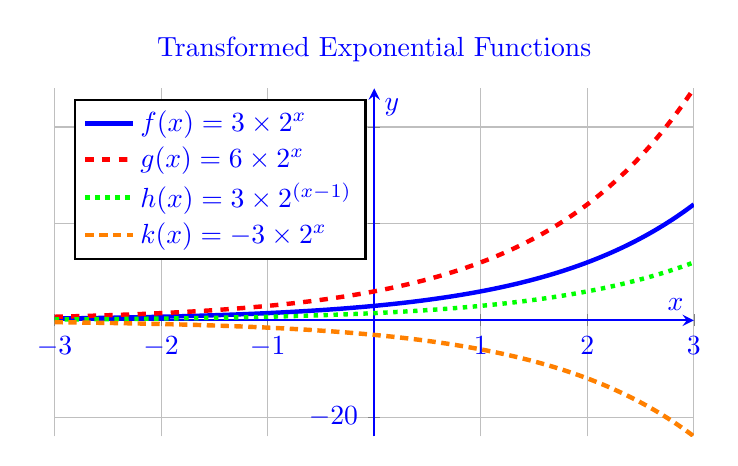
\begin{tikzpicture}
        \begin{axis}[
            xlabel={$x$},
            ylabel={$y$},
            grid=major,
            axis lines=middle,
            width=0.8\linewidth,
            height=6cm,
            title={Transformed Exponential Functions},
            legend pos=north west,
            domain=-3:3,
            samples=100,
            smooth,
            blue,
            thick,
            every axis plot/.append style={ultra thick},
            legend cell align=left,
        ]
            \addplot [blue] {3 * 2^x};
            \addlegendentry{$f(x) = 3 \times 2^x$}
            
            \addplot [red, dashed] {6 * 2^x};
            \addlegendentry{$g(x) = 6 \times 2^x$}
            
            \addplot [green, dotted] {3 * 2^(x - 1)};
            \addlegendentry{$h(x) = 3 \times 2^{(x - 1)}$}
            
            \addplot [orange, densely dashed] {-3 * 2^x};
            \addlegendentry{$k(x) = -3 \times 2^x$}
        \end{axis}
    \end{tikzpicture}
    \caption{Transformed Exponential Functions}
    \label{fig:transformed-exponential}
\end{figure}
    \end{enumerate}
\end{enumerate}
\end{lesson}
\begin{note}
    When considering the function \(y=a^x\):

    \textbf{Exponential Growth:} If $a > 1$, the function exhibits exponential growth. In this case, as $x$ increases, the corresponding values of $y$ grow rapidly.

    \textbf{Exponential Decay:} If $0 < a < 1$, the function demonstrates exponential decay. In such instances, as $x$ increases, the values of $y$ diminish rapidly, showcasing a decay behavior.
\end{note}
\newpage

\title{Geometry and Trigonometry: Unit 5}
\author{Kensukeken}
\date{December 2023}
\maketitle

\section{Unit 5: Trignometric Ratios}
\subsection{Basic Geometry}
In this section, we will explore fundamental concepts in geometry.

\textbf{Euclidean Geometry}
Euclidean geometry is the study of flat space.

\begin{theorem}
The sum of angles in a triangle is always $180^\circ$.
\end{theorem}

\begin{proof}
This follows from the parallel postulate.
\end{proof}

\subsection{Trigonometry}
Now, let's delve into trigonometry.

\subsection{Trigonometric Functions}
Trigonometric functions relate angles to the sides of a right triangle.

\begin{definition}
The sine function, denoted $\sin$, is defined as the ratio of the opposite side to the hypotenuse.
\end{definition}

\begin{example}
For a right triangle with an angle of $30^\circ$, if the opposite side is $3$ and the hypotenuse is $6$, then $\sin(30^\circ) = \frac{3}{6} = \frac{1}{2}$.
\end{example}
\subsection{Primary Trigonometric Ratios}

The primary trigonometric ratios in a right triangle are defined as follows:

\begin{align*}
\sin(\theta) &= \frac{\text{opposite}}{\text{hypotenuse}} \\
\cos(\theta) &= \frac{\text{adjacent}}{\text{hypotenuse}} \\
\tan(\theta) &= \frac{\text{opposite}}{\text{adjacent}}
\end{align*}

\textbf{Example:} Consider a right triangle with an angle $\theta$ such that $\sin(\theta) = \frac{3}{5}$. Find $\cos(\theta)$ and $\tan(\theta)$.

\textbf{Solution:}
Using the fact that $\sin^2(\theta) + \cos^2(\theta) = 1$, we can find $\cos(\theta)$:
\begin{align*}
\cos^2(\theta) &= 1 - \sin^2(\theta) \\
\cos(\theta) &= \pm \sqrt{1 - \sin^2(\theta)}
\end{align*}
Since $\theta$ is in the first quadrant, $\cos(\theta) = \sqrt{1 - \frac{9}{25}} = \frac{4}{5}$.
Now, use the definition of $\tan(\theta)$ to find $\tan(\theta)$:
\[\tan(\theta) = \frac{\sin(\theta)}{\cos(\theta)} = \frac{3/5}{4/5} = \frac{3}{4}\]

\subsection{Reciprocal Trigonometric Ratios}

The reciprocal trigonometric ratios are defined as the reciprocals of the primary trigonometric ratios:

\begin{align*}
\csc(\theta) &= \frac{1}{\sin(\theta)} \\
\sec(\theta) &= \frac{1}{\cos(\theta)} \\
\cot(\theta) &= \frac{1}{\tan(\theta)}
\end{align*}

\textbf{Example:} If $\sec(\theta) = \frac{5}{3}$, find $\sin(\theta)$.

\textbf{Solution:}
Since $\sec(\theta) = \frac{1}{\cos(\theta)}$, we can find $\cos(\theta)$ first:
\[\cos(\theta) = \frac{1}{\sec(\theta)} = \frac{3}{5}\]
Now, use the definition of $\sin(\theta)$:
\[\sin(\theta) = \frac{\text{opposite}}{\text{hypotenuse}} = \frac{\sqrt{5^2 - 3^2}}{5} = \frac{4}{5}\]

\subsection{Solving Right Triangles}

To solve a right triangle, you need to find the lengths of all sides and the measures of all angles. Use the primary and reciprocal trigonometric ratios to relate the angles and side lengths.

\textbf{Example:} In a right triangle, if $\sin(\alpha) = \frac{4}{5}$, find $\cos(\alpha)$ and $\tan(\alpha)$.

\textbf{Solution:}
Using the fact that $\cos(\alpha) = \sqrt{1 - \sin^2(\alpha)}$ and $\tan(\alpha) = \frac{\sin(\alpha)}{\cos(\alpha)}$, we can calculate:
\[\cos(\alpha) = \frac{3}{5}, \quad \tan(\alpha) = \frac{4}{3}\]

\subsection{Solving Oblique Triangles}

For oblique triangles (non-right triangles), the Law of Sines and Law of Cosines are used:

\subsection{Sine Law}

The Law of Sines states that for any triangle:

\[\frac{\sin(A)}{a} = \frac{\sin(B)}{b} = \frac{\sin(C)}{c}\]

\textbf{Example:} In triangle $ABC$, $a = 8$, $b = 11$, and $\angle C = 35^\circ$. Find the length of side $c$.

\textbf{Solution:}
Using the Law of Sines, we have:
\[\frac{\sin(C)}{c} = \frac{\sin(A)}{a} \implies c = \frac{\sin(C) \cdot a}{\sin(A)}\]
Substitute the given values to find $c$.

\subsection{Cosine Law}

The Law of Cosines relates the lengths of the sides of a triangle to the cosine of one of its angles:

\[c^2 = a^2 + b^2 - 2ab\cos(C)\]

\textbf{Example:} In triangle $XYZ$, $x = 7$, $y = 9$, and $\angle Z = 120^\circ$. Find the length of side $z$.

\textbf{Solution:}
Using the Law of Cosines, we have:
\[z^2 = x^2 + y^2 - 2xy\cos(Z)\]
Substitute the given values to find $z$.

\subsection{Challenging Problems}

\textbf{Problem 1:} In triangle $PQR$, $p = 10$, $q = 15$, and $\angle R = 45^\circ$. Find the lengths of sides $r$ and $s$.

\textbf{Problem 2:} In triangle $LMN$, $l = 12$, $\angle M = 30^\circ$, and $\angle N = 105^\circ$. Find the lengths of sides $m$ and $n$.

\textbf{Problem 3:} In triangle $ABC$, $a = 6$, $b = 8$, and $\angle C = 90^\circ$. Find the lengths of sides $c$ and $d$, where $d$ is the altitude from $\angle C$ to side $AB$.
\newpage

\subsection{Trigonometric equation}
\begin{minipage}[h]{0.5\textwidth}
    \trigfuns[2]{30}{\theta}
\end{minipage}%
\vspace{5em}
\begin{minipage}[h]{0.5\textwidth}
    \textbf{Pythagorean identity}\\ 
    $\sin^2 \theta + \cos^2 \theta =1$ \\
    $\tan \theta= \frac{\sin \theta}{\cos \theta}$\\
    $\tan \theta= $ Slope.\\
    \\\\
    Angles in standard position means $0^{\circ}$ is the position x-axis and positive angles move counter-clockwise, negative angles move clockwise.
\end{minipage}
\vspace{2em}
\textbf{Ex.1:} Show the following angles:

\begin{minipage}[h]{0.5\textwidth}
    \begin{enumerate}[label=(\alph*)]
        \item 
        \begin{tikzpicture}[
            > = Straight Barb,
            phasor/.style = {very thick, -{Stealth}},
            angles/.style = {draw, <->, angle eccentricity=1, right, angle radius=6mm, color=blue!70!cyan}
        ]
            % coordinates
            \draw[->] (-2.2,0) -- (2,0) coordinate (x) node[below left] {$x$};
            \draw[->] (0,-1.5) -- (0,2) node[below left] (y) {$y$};
            % phasors
            \draw[phasor, black] (0,0) -- (30:2.5) coordinate (v)  node[right,text=black] {$\mathbf{A}$};
            % angles drawn by pic
            \coordinate (X) at (0,0);
            \draw pic["$ \theta = 30^{\circ} $",angles,text=blue!70!cyan] {angle=x--X--v};
        \end{tikzpicture}
    \end{enumerate}
\end{minipage}%
\begin{minipage}[h]{0.5\textwidth}
    \begin{enumerate}[label=(\alph*),resume]
        \item 
        \begin{tikzpicture}[
            > = Straight Barb,
            phasor/.style = {very thick, -{Stealth}},
            angles/.style={draw, <->, angle eccentricity=1, right, angle radius=6mm, color=blue!70!cyan}]
            % coordinates
            \draw [->] (-2.2,0) -- (2,0) coordinate (x) node[below left] {$x$};
            \draw [->] (0,-1.5) -- (0,2) coordinate (y) node[below left] {$y$};
            % phasors
            \draw [phasor,black] (0,0) -- (-30:2.5) coordinate (v) node[left,text=black, yshift=-0.3cm] {$\mathbf{B}$};
            % angles drawn by pic
            \coordinate (X) at (0,0);
            \draw pic["$ \theta = -30^{\circ} $",angles,text=blue!70!cyan, yshift=-0.2cm, rotate around={-20:(X)}] {angle=v--X--x};
        \end{tikzpicture}
    \end{enumerate}
    \vspace{2em}
\end{minipage}
\textbf{Coterminal angles:} Angles in standard position that have the same terminal arms. \\ \\
For example: $30^{\circ}, 390^{\circ}$ and $-330^{\circ}$ are all coterminaz angles.

\newpage
\subsection{Unit Circle}
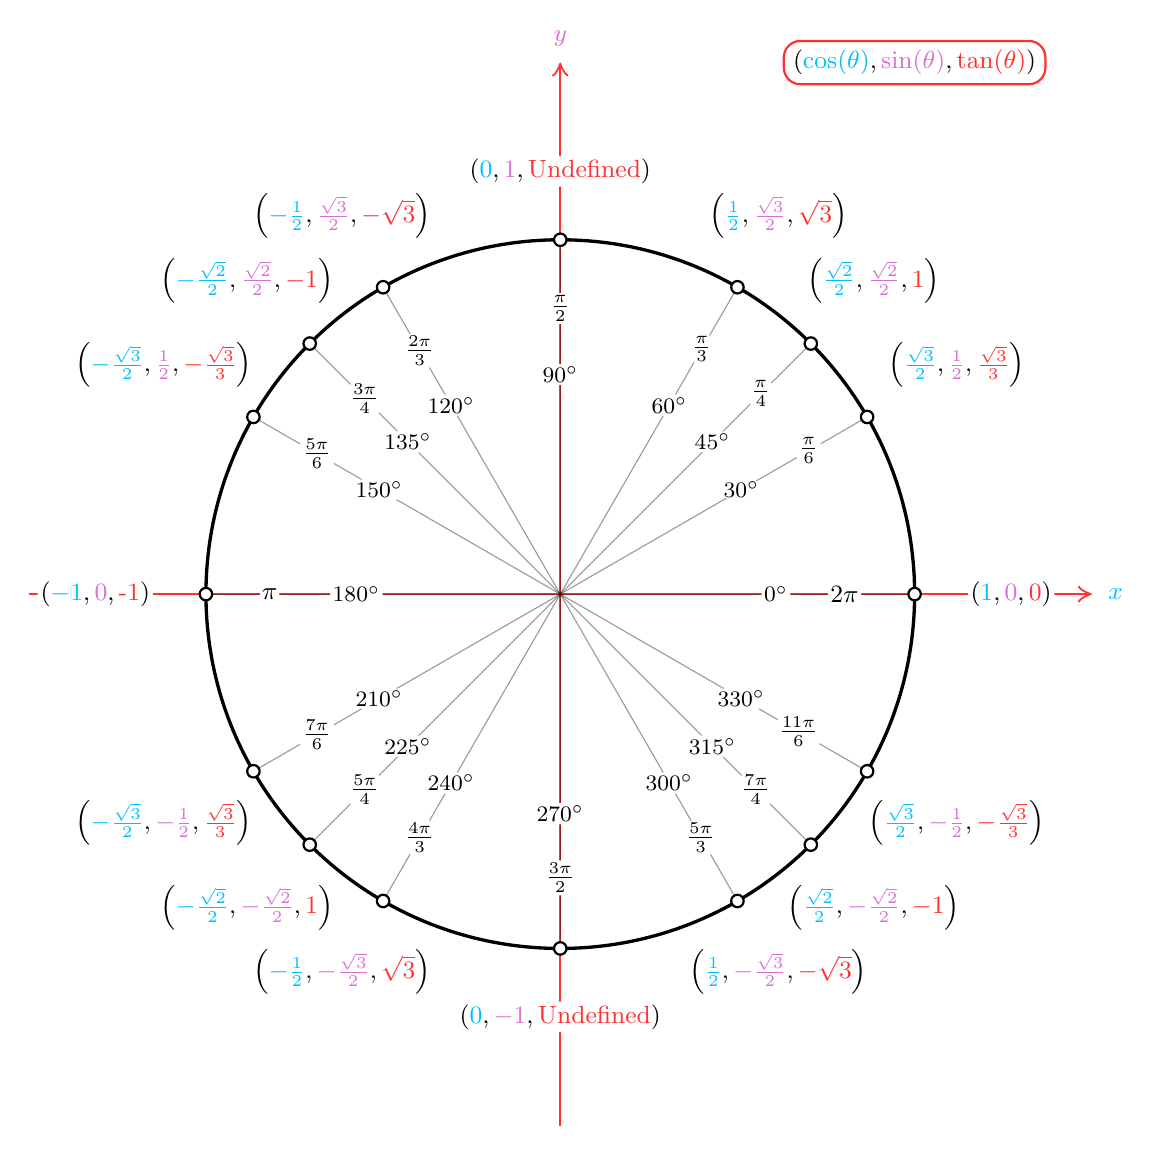
\begin{tikzpicture}[scale=4.5, font=\small]
    \definecolor{r}{HTML}{ff3030}
    \definecolor{b}{HTML}{00bfff}
    \definecolor{o}{HTML}{DA70D6}
    \def\angles{
        0/2\pi/1/0/0,
        30/\frac{\pi}{6}/\frac{\sqrt{3}}{2}/\frac{1}{2}/\frac{\sqrt{3}}{3},
        45/\frac{\pi}{4}/\frac{\sqrt{2}}{2}/\frac{\sqrt{2}}{2}/1,
        60/\frac{\pi}{3}/\frac{1}{2}/\frac{\sqrt{3}}{2}/\sqrt{3},
        90/\frac{\pi}{2}/0/1/\text{Undefined},
        120/\frac{2\pi}{3}/-\frac{1}{2}/\frac{\sqrt{3}}{2}/-\sqrt{3},
        135/\frac{3\pi}{4}/-\frac{\sqrt{2}}{2}/\frac{\sqrt{2}}{2}/-1,
        150/\frac{5\pi}{6}/-\frac{\sqrt{3}}{2}/\frac{1}{2}/-\frac{\sqrt{3}}{3},
        180/\pi/-1/0/\text{-1},
        210/\frac{7\pi}{6}/-\frac{\sqrt{3}}{2}/-\frac{1}{2}/\frac{\sqrt{3}}{3},
        225/\frac{5\pi}{4}/-\frac{\sqrt{2}}{2}/-\frac{\sqrt{2}}{2}/1,
        240/\frac{4\pi}{3}/-\frac{1}{2}/-\frac{\sqrt{3}}{2}/\sqrt{3},
        270/\frac{3\pi}{2}/0/-1/\text{Undefined},
        300/\frac{5\pi}{3}/\frac{1}{2}/-\frac{\sqrt{3}}{2}/-\sqrt{3},
        315/\frac{7\pi}{4}/\frac{\sqrt{2}}{2}/-\frac{\sqrt{2}}{2}/-1,
        330/\frac{11\pi}{6}/\frac{\sqrt{3}}{2}/-\frac{1}{2}/-\frac{\sqrt{3}}{3}
    }
    \begin{scope}[every node/.style={inner sep=1pt, outer sep=0pt}]
        \foreach \a/\at/\x/\y/\t in \angles {
            \begin{pgfinterruptboundingbox}
                \node (x) at (\a : 1.15) [anchor=\a-180] {\phantom{$\textstyle\left({\color{b} \x}, {\color{o} \y}, {\color{r} \t}\right)$}};
                \clip [rounded corners] (x.south west) rectangle (x.north east) (-1.6, -1.6) -- (1.6, -1.6) -- (1.6, 1.6) -- (-1.6, 1.6) -- cycle;
                \node (x) at (\a : 0.85) [anchor=\a] {\phantom{$\textstyle\at$}};
                \clip [rounded corners] (x.south west) rectangle (x.north east) (-1.6, -1.6) -- (1.6, -1.6) -- (1.6, 1.6) -- (-1.6, 1.6) -- cycle;
                \node (x) at (\a : 0.65) [anchor=\a, font=\footnotesize] {\phantom{$\textstyle\a^\circ$}};
                \clip [rounded corners] (x.south west) rectangle (x.north east) (-1.6, -1.6) -- (1.6, -1.6) -- (1.6, 1.6) -- (-1.6, 1.6) -- cycle;
                \clip (\a : 1) circle [radius=.5pt] (-1.6, -1.6) -- (-1.6, 1.6) -- (1.6, 1.6) -- (1.6, -1.6) -- cycle;
            \end{pgfinterruptboundingbox}
        }

        \draw [r, thick] (-1.5, 0) edge [-{Classical TikZ Rightarrow[length=5pt, width=6pt]}] (1.5, 0) node at (1.5, 0) [right=5pt] {$\textstyle\color{b} x$}
        (0, -1.5) edge [-{Classical TikZ Rightarrow[length=5pt, width=6pt]}] (0, 1.5) node at (0, 1.5) [above=5pt] {$\textstyle\color{o} y$};
        \draw [very thick] (0, 0) circle [radius=1];

        \foreach \a/\at/\x/\y/\t in \angles { \draw [opacity=.4] (0, 0) -- (\a : 1); }
    \end{scope}

    \scoped [every node/.style={inner sep=1pt, outer sep=0pt}] {
        \foreach \a/\at/\x/\y/\t in \angles {
            \node at (\a : 1.15) [anchor=\a-180, rounded corners] {$\textstyle\left({\color{b} \x}, {\color{o} \y}, {\color{r} \t}\right)$};
            \node at (\a : 0.85) [anchor=\a, rounded corners] {$\textstyle\at$};
            \node at (\a : 0.65) [anchor=\a, rounded corners, font=\footnotesize] {$\textstyle\a^\circ$};
            \draw [thick] (\a : 1) circle [radius=.5pt];
        }
    }

    \node at (1, 1.5) [thick, draw=r, rounded corners=6pt] {$\textstyle\left({\color{b} \cos(\theta)}, {\color{o} \sin(\theta)}, {\color{r} \tan(\theta)}\right)$};
\end{tikzpicture}


\newpage
\subsection{Trigonometric Ratios for Special Angles}

\subsection{Special Angles}
In trigonometry, certain angles have special significance due to their simplicity and exact values. The primary special angles are 0°, 30°, 45°, 60°, and 90°.

\subsubsection*{0° (Zero Degrees)}
\begin{minipage}{0.5\textwidth}
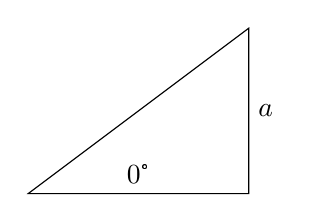
\begin{tikzpicture}[scale=0.7]
    \draw (0,0) -- (4,0) -- (4,3) -- cycle;
    \node[above] at (2,0) {0\textdegree};
    \node[right] at (4,1.5) {$a$};
\end{tikzpicture}
\end{minipage}%
\begin{minipage}{0.5\textwidth}
\[
\begin{aligned}
\sin(0^\circ) &= 0, \\
\cos(0^\circ) &= 1, \\
\tan(0^\circ) &= 0.
\end{aligned}
\]
\end{minipage}

\subsubsection*{30°}
\begin{minipage}{0.5\textwidth}
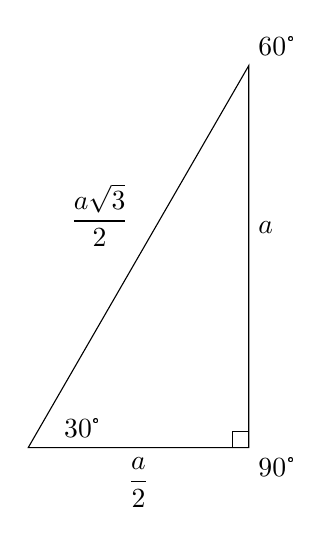
\begin{tikzpicture}[scale=0.7]
    \draw (0,0) -- (4,0) -- (4,{4*sqrt(3)}) -- cycle;
    \draw (3.7,0) -- (3.7,0.3) -- (4,0.3);
    \node[above left] at (1.5,0) {30\textdegree};
    \node[above right] at (4,{4*sqrt(3)}) {60\textdegree};
    \node[below right] at (4,0) {90\textdegree};
    \node[right] at (4,4) {$a$};
    \node[below] at (2,0) {$\dfrac{a}{2}$};
    \node[above left] at (2,{2*sqrt(3)}) {$\dfrac{a\sqrt{3}}{2}$};
\end{tikzpicture}
\end{minipage}%
\begin{minipage}{0.5\textwidth}
\[
\begin{aligned}
\sin(30^\circ) &= \dfrac{1}{2}, \\
\cos(30^\circ) &= \dfrac{\sqrt{3}}{2}, \\
\tan(30^\circ) &= \dfrac{1}{\sqrt{3}}.
\end{aligned}
\]
\end{minipage}

\subsubsection*{45°}
\begin{minipage}{0.5\textwidth}
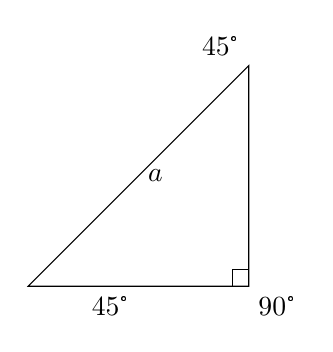
\begin{tikzpicture}[scale=0.7]
    \draw (0,0) -- (4,0) -- (4,4) -- cycle;
    \draw (3.7,0) -- (3.7,0.3) -- (4,0.3);
    \node[below left] at (2,0) {45\textdegree};
    \node[above left] at (4,4) {45\textdegree};
    \node[below right] at (4,0) {90\textdegree};
    \node[right] at (2,2) {$a$};
\end{tikzpicture}
\end{minipage}%
\begin{minipage}{0.5\textwidth}
\[
\begin{aligned}
\sin(45^\circ) &= \dfrac{\sqrt{2}}{2}, \\
\cos(45^\circ) &= \dfrac{\sqrt{2}}{2}, \\
\tan(45^\circ) &= 1.
\end{aligned}
\]
\end{minipage}

\subsubsection*{60°}
\begin{minipage}{0.5\textwidth}
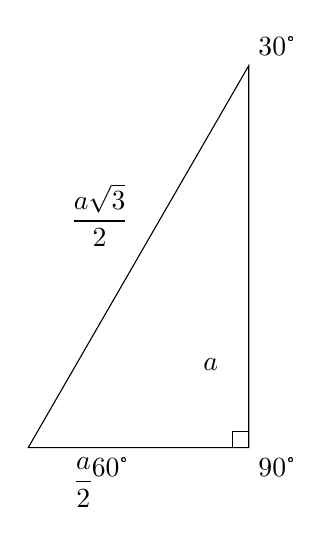
\begin{tikzpicture}[scale=0.7]
    \draw (0,0) -- (4,0) -- (4,{4*sqrt(3)}) -- cycle;
    \draw (3.7,0) -- (3.7,0.3) -- (4,0.3);
    \node[below left] at (2,0) {60\textdegree};
    \node[above right] at (4,{4*sqrt(3)}) {30\textdegree};
    \node[below right] at (4,0) {90\textdegree};
    \node[right] at (3,1.5) {$a$};
    \node[below] at (1,0) {$\dfrac{a}{2}$};
    \node[above left] at (2,{2*sqrt(3)}) {$\dfrac{a\sqrt{3}}{2}$};
\end{tikzpicture}
\end{minipage}%
\begin{minipage}{0.5\textwidth}
\[
\begin{aligned}
\sin(60^\circ) &= \dfrac{\sqrt{3}}{2}, \\
\cos(60^\circ) &= \dfrac{1}{2}, \\
\tan(60^\circ) &= \sqrt{3}.
\end{aligned}
\]
\end{minipage}

\subsubsection*{90°}
\begin{minipage}{0.5\textwidth}
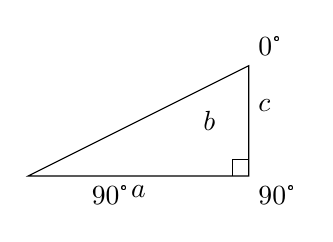
\begin{tikzpicture}[scale=0.7]
    \draw (0,0) -- (4,0) -- (4,2) -- cycle;
    \draw (3.7,0) -- (3.7,0.3) -- (4,0.3);
    \node[below left] at (2,0) {90\textdegree};
    \node[above right] at (4,2) {0\textdegree};
    \node[below right] at (4,0) {90\textdegree};
    \node[right] at (3,1) {$b$};
    \node[below] at (2,0) {$a$};
    \node[above right] at (4,1) {$c$};
\end{tikzpicture}
\end{minipage}%
\begin{minipage}{0.5\textwidth}
\[
\begin{aligned}
\sin(90^\circ) &= 1, \\
\cos(90^\circ) &= 0 \, (\text{undefined}), \\
\tan(90^\circ) &= \infty \, (\text{undefined}).
\end{aligned}
\]
\end{minipage}

\subsection{Coterminal Angles:}
Coterminal angles are angles that share the same initial and terminal sides but can differ by integer multiples of a full revolution (360° or $2\pi$ radians). Two angles $\theta$ and $\theta + 360n$ (where $n$ is an integer) are coterminal.

\subsection{Principal Angles:}
The principal angle is the smallest positive angle between the terminal side of an angle and the x-axis. For any angle $\theta$, the principal angle $\theta_p$ is given by:
\[ \theta_p = \theta - 360n \]
\newpage
\subsection{Trig identities}
An identity is an equation which is true for all values of the variable. 
\subsection{Reciprocal identity}
\begin{align*}
\csc(\theta) &= \frac{1}{\sin(\theta)} \\
\sec(\theta) &= \frac{1}{\cos(\theta)} \\
\cot(\theta) &= \frac{1}{\tan(\theta)}
\end{align*}
\subsection{Pythagorean identity}

$$\cos^2\theta +\sin^2\theta =1\\$$

\subsubsection*{Rearranging Pythagorean identity}
\begin{align*}
    \cos^2\theta +\sin^2\theta =1\\
    \cos^2\theta =1-\sin^2\theta\\
    \sin^2\theta=1-\cos^2\theta
\end{align*}
\subsection{Quotient identity:}
\[\tan\theta =\frac{\sin \theta}{\cos \theta} \quad \text{and } \quad \cot\theta=\frac{\cos\theta}{\sin\theta}\]
\subsection*{Steps to prove identities}
\begin{enumerate}
    \item Simplify one side at a time (Both sides is not allowed.)
    \item Start with more complicated side first.
    \item Simplify one side as much as you can, if you get stuck than switch to take other side.
    \item Converting everything into sine and cos is sometimes helpful.
    \item Use your intuition!
\end{enumerate}
\newpage

\section{Unit 6: Sinusoidal Functions}

\begin{tcolorbox}[mybox]
Sinusoidal function are periodic function where graph looks like smooth symmetical waves, where any potion can be horizontally translated onto another potion of curve. \\
Graph of sinusdidal function can be created by transforming $y=\sin{\theta}$ and $y=\cos{\theta}$.\\

    A periodic function is a function that repeats its values in regular intervals. In this document, we will explore the properties and examples of periodic functions.\\
    Note: sinusoidal function are all period function but period function are not sinusoidal.
    
\end{tcolorbox}

\begin{center}
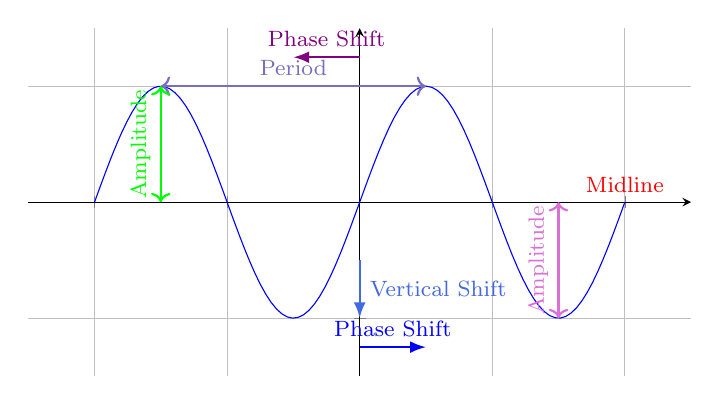
\begin{tikzpicture}
\begin{axis}[
    axis lines=middle,
    xticklabels={},
    yticklabels={},
    xtick={-2*pi,-pi,0,pi,2*pi},
    ytick={-2,0,2},
    grid=major,
    ymin=-3,
    ymax=3,
    xmin=-2.5*pi,
    xmax=2.5*pi,
    width=10cm,
    height=6cm
]
\addplot[domain=-2*pi:2*pi, samples=100, color=blue]{2*sin(deg(x))};
\draw[dashed] (axis cs:-2*pi,0)--(axis cs:2*pi,0);
\node[align=center, font=\footnotesize, color=red] at (axis cs:2*pi,0.3){Midline};
\draw[<->, Periwinkle, thick] (axis cs:pi/2,2.0)--(axis cs:-3*pi/2,2.0) node[midway,above,font=\footnotesize]{Period};
\draw[<->, green, thick] (axis cs:-1.5*pi,0)--(axis cs:-1.5*pi,2) node[midway,left,font=\footnotesize,rotate=90,above]{Amplitude};
\draw[<->, Orchid, thick] (axis cs:1.5*pi,-2)--(axis cs:1.5*pi,0) node[midway,right,font=\footnotesize,rotate=-270,above]{Amplitude};
\draw[-{Latex[length=2mm]}, Purple, thick] (axis cs:0,2.5)--(axis cs:-pi/2,2.5) node[midway,above,font=\footnotesize]{Phase Shift};
\draw[-{Latex[length=2mm]}, blue, thick] (axis cs:0,-2.5)--(axis cs:pi/2,-2.5) node[midway,above,font=\footnotesize]{Phase Shift};
\draw[-{Latex[length=2mm]}, RoyalBlue, thick] (axis cs:0,-1)--(axis cs:0,-2) node[midway,right,font=\footnotesize]{Vertical Shift};
\end{axis}
\end{tikzpicture}
\end{center}


Midline, amplitude, and period are three features of sinusoidal graphs.
\newpage
\subsection{Characteristics of Sinusoidal Graphs}
\subsection{Midline/Axis of the Curve:}
The \textcolor{Maroon}{\underline{midline}} is a horizontal line right in the middle between the highest and lowest points of the graph. It's calculated using the formula:
\[y = \frac{\text{max value + min value}}{2}\]

\subsection{Amplitude:}
The \textcolor{LimeGreen}{\underline{amplitude}} is how high or low the graph reaches from the middle line. You find it using:
\[a = \frac{\text{max value - min value}}{2}\]

\subsection{Period:}
The \textcolor{Periwinkle}{\underline{period}} is how wide one complete cycle of the graph is. It's found by looking at the distance between two consecutive high or low points. The formula is:
\[P = \frac{2\pi}{k}\quad \text{or} \quad P = \frac{360}{k} \]

\subsection{Phase Shift:}
The \textcolor{Purple}{\underline{phase shift}} is like a sideways movement of the graph, showing if it's shifted left or right. For \(y = A \sin(k \theta + d) + C\), you calculate it using:
\[\text{Horizontal shift} = \frac{d}{k} \text{ or }  -\frac{d}{k}\]

\subsection{Vertical Shift:}
The \textcolor{RoyalBlue}{\underline{vertical shift}} is like lifting or lowering the whole graph. For \(y = A \sin(k \theta + d) + C\), it shifts the entire graph up or down by \(C\) units.

\subsection{Key Intervals:}
\textcolor{OliveGreen}{\underline{Key intervals}} are specific ranges of values where the graph undergoes significant changes. These intervals are essential for identifying crucial points, such as the highest and lowest values, contributing to a better understanding of the function's behavior.

One important key interval is $\frac{\text{Period}}{4}$, representing a quarter of the period. It marks a position in the graph where distinctive shifts and changes occur, aiding in the analysis of the function's characteristics.

\subsection{Trigonometric Functions}
The graphs of $y=\sin\theta, y=\cos\theta, y=\tan\theta.$ are shown below.
\begin{figure}[h]
    \centering
    \includegraphics[width=1.0\textwidth]{Unit 6/sin-cos-tan.png}
\end{figure}
\subsection{Transformations of Trigonometric Functions}
\begin{itemize}
    \item Transformations apply to trig functions as they do to any other function.
    \item The graphs of $y=a \sin k(\theta+d)+c$ and $y=a \cos k(\theta+b)+d$ are transformations of the graphs $y=\sin \theta$ and $y=\cos \theta$ respectively.
    \item The value of $a$ determines the vertical stretch, called the amplitude. It also tells whether the curve is reflected in the $\theta$-axis.
    \item The value of $k$ determines the horizontal stretch. The graph is stretched by a factor of $\frac{1}{k}$. We can use this value to determine the period of the transformation of $y=\sin \theta$ or $y=\cos \theta$.
    \item The period of $y=\sin k \theta$ or $y=\cos k \theta$ is $\frac{360^{\circ}}{k}, k>0$. The period of $y=\tan k \theta$ is $\frac{180^{\circ}}{k}, k>0$.
    \item The value of $d$ determines the horizontal translation, known as the phase shift.
    \item The value of $\mathrm{c}$ determines the vertical translation. $y=d$ is the equation of the axis of the curve.
\end{itemize}

\subsection*{Examples}
\begin{itemize}
    \item 
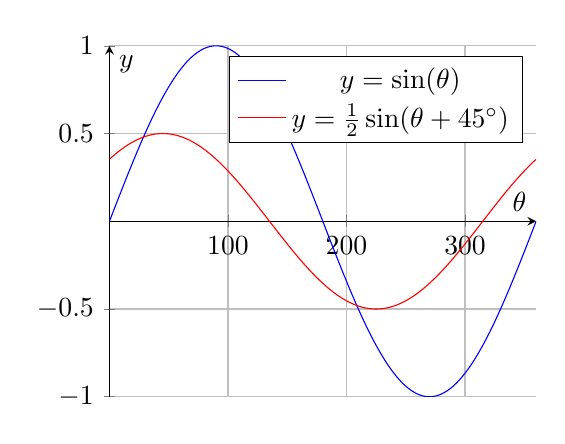
\begin{tikzpicture}
    \begin{axis}[
        domain=0:360, % Assuming you want to plot over one full revolution (0 to 360 degrees)
        samples=500, % Number of samples for a smooth curve
        xlabel={$\theta$},
        ylabel={$y$},
        legend pos=north east,
        grid=both,
        axis lines=middle
    ]

    % Plot y = sin(theta) and y = 0.5*sin(theta + 45)
    \addplot[blue, smooth] {sin(x)};
    \addlegendentry{$y = \sin(\theta)$}

    \addplot[red, smooth] {0.5*sin(x + 45)};
    \addlegendentry{$y = \frac{1}{2}\sin(\theta + 45^\circ)$}

    \end{axis}
\end{tikzpicture}
\item 
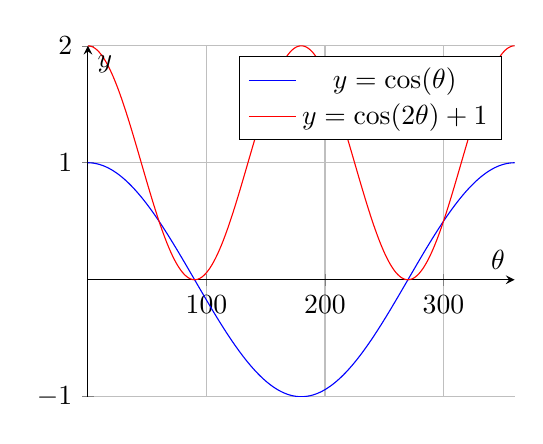
\begin{tikzpicture}
    \begin{axis}[
        domain=0:360, % Assuming you want to plot over one full revolution (0 to 360 degrees)
        samples=500, % Number of samples for a smooth curve
        xlabel={$\theta$},
        ylabel={$y$},
        legend pos=north east,
        grid=both,
        axis lines=middle
    ]

    % Plot y = cos(theta) and y = cos(2*theta) + 1
    \addplot[blue, smooth] {cos(x)};
    \addlegendentry{$y = \cos(\theta)$}

    \addplot[red, smooth] {cos(2*x) + 1};
    \addlegendentry{$y = \cos(2\theta) + 1$}

    \end{axis}
\end{tikzpicture}
\end{itemize}
\newpage
\subsection{Property of Sine function }
\begin{tabular}{|c|c|}
\hline
\textbf{Property} & \(y = \sin(x)\) \\
\hline
Amplitude & 1 \\
\hline
Period & \(360^\circ\) \\
\hline
Equation of Axis & \(y = 0\) \\
\hline
Domain & \(\{x | x \in \mathbb{R}\}\) \\
\hline
Range & \(\{y \in \mathbb{R} | -1 \leq y \leq 1\}\) \\
\hline
x-intercepts & \(x \in \{180n, n \in \mathbb{Z}\}\) \\
\hline
y-intercept & 0 \\
\hline
Maximum & \(1, \text{when } x \in \{90 + 360n, n \in \mathbb{Z}\}\) \\
\hline
Minimum & \(-1, \text{when } x \in \{270 + 360n, n \in \mathbb{Z}\}\) \\
\hline
Intervals of increase & \(90 < x < 270, \text{and all intervals obtained by adding } 360n, n \in \mathbb{Z}\) \\
\hline
Intervals of decrease & \(270 < x < 90, \text{and all intervals obtained by adding } 360n, n \in \mathbb{Z}\) \\
\hline
\end{tabular}

\subsection{Property of Cosine function}
\begin{tabular}{|c|c|}
\hline
\textbf{Property} & \(y = \cos(x)\) \\
\hline
Amplitude & 1 \\
\hline
Period & \(360^\circ\) \\
\hline
Equation of Axis & \(y = 0\) \\
\hline
Domain & \(\{x | x \in \mathbb{R}\}\) \\
\hline
Range & \(\{y \in \mathbb{R} | -1 \leq y \leq 1\}\) \\
\hline
x-intercepts & \(x \in \{90 + 180n, n \in \mathbb{Z}\}\) \\
\hline
y-intercept & 1 \\
\hline
Maximum & \(1, \text{when } x \in \{360n, n \in \mathbb{Z}\}\) \\
\hline
Minimum & \(-1, \text{when } x \in \{180 + 360n, n \in \mathbb{Z}\}\) \\
\hline
Intervals of increase & \(0 < x < 180, \text{and all intervals obtained by adding } 360n, n \in \mathbb{Z}\) \\
\hline
Intervals of decrease & \(180 < x < 360, \text{and all intervals obtained by adding } 360n, n \in \mathbb{Z}\) \\
\hline
\end{tabular}
\newpage


\newpage
% Extras
\section*{Extra}
\subsection*{Definition}

A function $f(x)$ is periodic with period $T$ if, for all $x$ in the domain of $f$, the following holds:

\[
f(x + T) = f(x)
\]

This means that the function values repeat every $T$ units along the $x$-axis.

\subsection*{Examples}

\subsubsection*{Sine Function}

\begin{tcolorbox}[mybox]
    The sine function, denoted by $\sin(x)$, is a classic example of a periodic function. Its period is $2\pi$, and the function is defined as:
    
    \[
    \sin(x) = \sum_{n=0}^{\infty} \frac{(-1)^n}{(2n+1)!} x^{2n+1}
    \]
\end{tcolorbox}

\begin{figure}[h]
    \centering
    \includegraphics[width=0.6\textwidth]{Unit 6/Sine-Graph.png}
    \caption{Graph of the sine function.}
\end{figure}
\newpage 
\subsubsection*{Square Wave}

\begin{tcolorbox}[mybox]
    The square wave is another example of a periodic function. It has a period $T$ and is defined as:
    
    \[
    \text{square wave}(x) = 
    \begin{cases} 
    1 & \text{if } 0 \leq x < \frac{T}{2} \\
    -1 & \text{if } \frac{T}{2} \leq x < T
    \end{cases}
    \]
\end{tcolorbox}

\begin{figure}[h]
    \centering
    \includegraphics[width=0.6\textwidth]{Unit 6/square_wave.JPG}
    \caption{Graph of a square wave.}
\end{figure}

\subsection*{Conclusion}

\begin{tcolorbox}[mybox]
    Periodic functions are essential in various branches of mathematics and physics. Understanding their properties and behavior is crucial for analyzing and modeling periodic phenomena.
\end{tcolorbox}

\tikzset{>=latex} 
\tikzset{axis/.style={black, thick,->}}
\tikzset{vector/.style={>=stealth,->}}
\tikzset{every text node part/.style={align=center}}
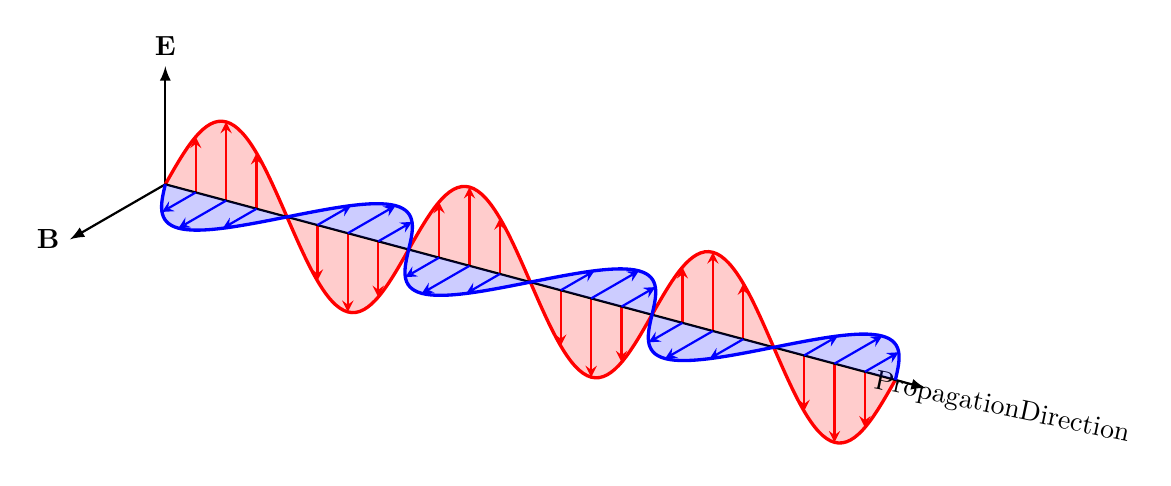
\begin{tikzpicture}[x={(-150:0.7)}, y={(90:1.0)}, z={(-15:8mm)}]
\def\wave{
    \draw[fill, very thick, fill opacity=.2]
         (0,0) sin (1,1) cos (2,0) sin (3,-1) cos (4,0)
               sin (5,1) cos (6,0) sin (7,-1) cos (8,0)
               sin (9,1) cos (10,0) sin (11,-1) cos (12,0);
         
    \foreach \shift in {0,4,8}
    {
        \begin{scope}[xshift=\shift cm,thin]
                \draw[-stealth, thick] (.5,0)  -- (0.5,0 |- 45:1cm);
                \draw[-stealth, thick] (1,0)   -- (1,1);
                \draw[-stealth, thick] (1.5,0) -- (1.5,0 |- 45:1cm);
                \draw[-stealth, thick] (2.5,0) -- (2.5,0 |- -45:1cm);
                \draw[-stealth, thick] (3,0)   -- (3,-1);
                \draw[-stealth, thick] (3.5,0) -- (3.5,0 |- -45:1cm);
         \end{scope}
    } 
}
\begin{scope}[canvas is zy plane at x=0, draw=red, fill=red] 
    \draw[-latex, thick, black] (0,0) -- (0, 1.5) node[above] {$\mathbf E$};
    \wave
\end{scope}
\begin{scope}[canvas is zx plane at y=0, draw=blue, fill=blue]
    %% Direction of Propagation
    \draw[-latex, thick, black] (0,0) -- (12.5, 0) node[rotate = -12, pos=1.1] {Propagation\\Direction};
    \draw[-latex, thick, black] (0,0) -- (0,2) node[left] {$\mathbf B$};
    \wave
\end{scope}
\end{tikzpicture}

\newpage
\section{Unit 7: Discrete Functions (Series and Sequences)}
\subsection{Arithmetic sequence}
\begin{lesson}{Discrete functions - Sequences and series}
    \begin{arrowlist}
        \item Sequence - An ordered list of numbers (e.g., $2, 5, 8, 11, \ldots$)
        \item Term - A number in a sequence (e.g., $t_1 =$ first term, $t_{10} =$ tenth term)
        \item Arithmetic sequence $\Rightarrow$ A sequence that has the same difference ($d$) between any pair of consecutive terms.

    \begin{example}
        \[\underbrace{2, 5, 8, 11, \ldots}_{\textcolor{blue}{\text{Common difference of 3}}}\]
    \end{example}

    \item General term - A formula, labeled $t_n$, that expresses each term of a sequence as a function of its position.

    \begin{example}
        $2, 4, 6, 8, 10, \ldots$ has a general term of $t_n = 2n$.\\
        \begin{align*}
            t_1 &=2(1) =2 \\
            t_4 &= 2(4) =8 \\
            t_{24} &=2(24) = 48
        \end{align*}
    \end{example}
    \item The general term for an arithmetic sequence is:
    \begin{center}
\begin{minipage}{0.4\textwidth}
\begin{equation*}
    t_n=a+(n-1)d
\end{equation*}
\end{minipage}%
\begin{minipage}{0.6\textwidth}
Where:
\begin{itemize}
    \item a is the first term.
    \item d is the common difference 
    \item n is the term \# 
\end{itemize}
\end{minipage}
\end{center}
\end{arrowlist}
\end{lesson}
\begin{example}
    \underline{\textbf{Ex.1:}}
    \begin{enumerate}[label=\alph*.]
        \item Find the general term for the arithmetic sequence:
        \item Find $t_9$ (the $9^{th}$ term)
    \end{enumerate}
    
    \begin{enumerate}[label=\roman*)]
        \item $10, 14, 18, 22, \ldots$
        \begin{enumerate}[label=\alph*.]
            \item 
            \begin{align*}
                &\text{\textcolor{blue}{Given:}} \quad a = 10 \text{ (first term)} \\
                &t_n = 10 + (n-1)(4)
            \end{align*}
            \item 
            \begin{align*}
                t_9 &= a + (9-1)d \\ 
                &= 10 + 8(4) \\ 
                &= 42 \\
                &\boxed{\therefore\ t_9 = 42}
            \end{align*}
        \end{enumerate}
        \item $-33, -23, -13, -3, 7, \ldots$
        \begin{enumerate}[label=\alph*.]
            \item 
            \begin{align*}
                &\text{\textcolor{blue}{Given:}} \quad a = -33 \text{ (first term)} \\
                &d = t_2 - t_1 \quad \text{\textcolor{blue}{(common difference)}} \\
                &= -23 - (-33) \\
                &= 10 \\
                &t_n = -33 + (n-1)(10) \\
                &= 10n - 43
            \end{align*}
            \item 
            \begin{align*}
                t_9 &= -33 + (9-1)(10) \\
                &= -33 + 8(10) \\
                &= -33 + 80 \\
                &= 47 \\
                &\boxed{\therefore\ t_9 = 47}
            \end{align*}
        \end{enumerate}
    \end{enumerate}
\end{example}
\begin{example}
    \underline{Ex.2:} Find the $33^{3rd}$ term in the sequence 18, 11, 4, -3, $\ldots$. \\ 
    Solution:
    \begin{align*}
        a &=10 \\
        d&= -7 && t_n=18+(n-1)(-7) \\ 
        t_{33}&=18+(33-1)(-7)\\
        &=18+(33)(-7)\\
        &=18-224\\
        & \boxed{t_{33}=-206}
    \end{align*}
\end{example}
\begin{example}
    \underline{Ex.3:} Find the \# of terms in the sequence.

\begin{center}
    \begin{minipage}{0.4\textwidth}
\begin{equation*}
    \underbrace{\text{31, 27}}_{\textcolor{red}{-4}}, \underbrace{\text{27, 23}}_{\textcolor{red}{-4}}, \underbrace{\text{23, 19}}_{\textcolor{red}{-4}}, \ldots, -53
\end{equation*}
        \vspace{1ex} 
        $\therefore$ \textcolor{red}{\text{arithmetic}}
    \end{minipage}%
    \begin{minipage}{0.6\textwidth}
        \begin{enumerate}
            \item Make a general term.
            \item Substitute in $-53$.
            \item Solve for $n$.
        \end{enumerate}
    \end{minipage}
\end{center}
\begin{align*}
    a &= 31, \quad d= -4 & 84 &= (n-1)(-4)\\
    t_n &= 31 + (n-1)(-4) & 21 &= n-1\\
    &\text{(sub in $-53$ for $t_n$)} \quad & 22 &= n \\
    -53 &= 31 + (n-1)(-4) & \therefore \quad & \text{There are 22 terms}\\
    &\text{(solve for $n$)}
\end{align*}
\end{example}
\newpage 
\begin{example}
    \underline{Ex.4} For an arithmetic sequence, $t_7=53$ and $t_n=97$. Find $t_{100}$.\\
    \underline{\textcolor{blue}{Solution \circled{1} :}}
    \begin{align*}
        t_7 &= \textcolor{red}{53} \quad && t_{11} = \textcolor{red}{97}  \\
        a + (n-1)d &= \textcolor{red}{53} \quad && a + (11-1)d = \textcolor{red}{97}  \\
        a + (7-1)d &= \textcolor{red}{53} \quad && a + 10d = \textcolor{red}{97} \quad \circled{2} \\
        a + 6d &= \textcolor{red}{53} \quad \circled{1}
    \end{align*}
  \begin{minipage}[t]{0.48\textwidth}
        $\begin{array}{ccccc}
             & \textcolor{blue}{\text{Using elimination}} \\
             & \textcolor{cyan}{\circled{2}} \quad a + 10d = \textcolor{orange}{97} \\
             & \textcolor{cyan}{\circled{1}} \quad a + 6d = \textcolor{orange}{53} \\
             \hline \
             & \quad \textcolor{purple}{4d = 44} \\
             & \quad \textcolor{purple}{d = 11}
        \end{array}$
        \begin{align*}
            &\textcolor{blue}{\text{Substitute }} d=11 \textcolor{blue}{\text{ into }} \textcolor{cyan}{\circled{1}} \\
            a + 6(11) &= \textcolor{orange}{53} \\
            a &= \textcolor{orange}{53 - 66} \\
            a &= \textcolor{orange}{-13}
        \end{align*}
    \end{minipage}%
    \begin{minipage}[t]{0.48\textwidth}
        \begin{align*}
            t_n &= \textcolor{orange}{-13 + (n-1)(11)} \\
            t_{100} &= \textcolor{orange}{-13 + (99)(11)} \\
            t_{100} &= \textcolor{orange}{1076} \\
        \end{align*}
        Once we found $d=11$,
        \begin{align*}
            t_7 + 93d &= \textcolor{orange}{t_{100}} \\
            \textcolor{red}{53 + 93(11)} &= \textcolor{orange}{t_{100}} \\
            t_{100} &= \textcolor{orange}{1076}
        \end{align*}
        Or,
        \begin{align*}
            t_{100} &= \textcolor{red}{t_{11}} + 89d \\
            &= \textcolor{red}{97 + 89(11)} \\
            &= \textcolor{orange}{1076}
        \end{align*}
    \end{minipage}
    \newpage
 \underline{\textcolor{blue}{Solution \circled{2} :}}
    \begin{align*}
        &\textcolor{purple}{\underbrace{t_{11}-t_7=4d}_{\text{proof}}}\\
        &(a+10d)(a+6d)\\
        &=10d-6d\\
        &=4d
    \end{align*}
    \begin{align*}
        t_{11}-t_7=4d && t_{100}=t_7+93d\\
        \textcolor{red}{97-53=4d} && =\textcolor{red}{53 +93(11)}\\
        \textcolor{purple}{44=4d} &&=\textcolor{purple}{1076} \\
        \textcolor{purple}{11=d}
    \end{align*}
\end{example}
\begin{example}
     \underline{Ex.5:} For an arithmetic sequence: $t_4=19$ and $t_{21}=-49$. Find $t_{38:}$\\
     \begin{align*}
         t_{21}-t_{4}&=17d && t_{38}=t_{21}+17d && t_{38}=t_{4}+34d\\
         -49-19&=17d &&=49+17(-4)&& =19+34(-4)\\
         -68&=17d && t_{38}=-117&& =-117\\
         -4&=d &
     \end{align*}
\end{example}
\newpage
\begin{lesson}{Arithmetic sequence (cont'd)}
    Recursive sequence $\Rightarrow$ a sequence for which one term(or more) is given and each successive term is determined from the previous term(s).\\ \\
    For an arithmetic formula sequence the recursive formula:
    \begin{equation*}
        \boxed{t_1=a,t_n=t_{n-1}+d, n \in \mathbb{N}, n>1}
    \end{equation*}
    \underline{\hl{Recall:}} 1, 1, 2, 3, 5, 8\\
    $$t_1=,t_2=1,t_n=t_{n-1}+t_{n+2}, n \in \mathbb{N}, n >2$$
\end{lesson}
\begin{example}
    \underline{Ex.1:} Write the recursive formula for each arithmetic sequence 
    \begin{enumerate}[label=\alph*.]
        \item 5,11,17,23, $\ldots$
        \begin{equation*}
            t_1=5, t_n=t_n=t_{n-1}+6, n \in \mathbb{N}, n>1
        \end{equation*}
        \item $\frac{1}{2}$, $\frac{-1}{2}$, $\frac{-3}{2}$, $\frac{-5}{2}$, $\ldots$
        \begin{equation*}
            t_1=\frac{1}{2}, t_n=t_n=t_{n-1}+1, n \in \mathbb{N}, n>1
        \end{equation*}        
    \end{enumerate}
\end{example}
\begin{example}
    \underline{Ex.2:} Write the first 4 terms of the sequence
    \begin{enumerate}[label=\alph*.]
        \item $t_1=80, t_n=t_{n-1}-8, n\in \mathbb{N}, n>1$
        \begin{equation*}
            80, 72, 64, 56, \ldots 
        \end{equation*}
    \end{enumerate}
\end{example}
\newpage
\subsection{Geometric sequence}
\begin{lesson}{Geometric sequence}
    \begin{arrowlist}
        \item Recursive sequence in which noew terms are created by multiplying the previous terms by the same value(common ratio).
    \end{arrowlist}
\end{lesson}
\begin{example}
    2, 6 , 18, 54, $\dots$\\
    a=2 first term \quad Common ratio (r)=3 since $\frac{t_2}{t_1}=\frac{t_3}{t_2}=\frac{t_4}{t_3}=3$
\end{example}
General term $\Rightarrow t_n=ar^{n-1}$ 
\begin{align*}
\therefore t_1&=ar^{1-1} && t_2=ar^{2-1} && t_3=ar^{3-1} && t_4=ar^{4-1} &&\text{AND} \\
t_1&=ar^{0} && t_2=ar^1 && t_3=ar^{2} && t_4=ar^3 && \text{SO} \\
t_1&=a && t_2=ar &&&&&& \text{ON!} \\
\end{align*}
\begin{equation*}
    \overbrace{a }^{\times \text{r}}, \overbrace{ar }^{\times \text{r}}, \overbrace{ar^2}^{\times \text{r}}, \overbrace{ar^3 }^{\times \text{r}}, \overbrace{ar^4 }^{\times \text{r}}, \ldots
\end{equation*}
\subsubsection*{Recursive Formula:}
\begin{equation*}
    t_1=,t_n=(t_{n-1})(r), n \in \mathbb{N}, n>1
\end{equation*}
\begin{example}
    \underline{Ex.1:} For the sequence: $2, 6, 18, 53$
    \begin{enumerate}[label=(\alph*), align=left, left=0pt, labelwidth=1.5em, labelsep=1em]
        \item Determine recursive formula: 
        \[
        t_1 = 2, \quad t_n = (t_{n-1}) (3), n \in \mathbb{N}, \; n > 1
        \]
        \item General term: 
        \[
        t_n = 2 (3)^{n-1}
        \]
        \item $t_{10}$
        \begin{align*}
            t_{10} &= 2 \cdot 3^{10-1} \\
                   &= 2 \cdot 3^9 \\
                   &= 39,366
        \end{align*}
    \end{enumerate}
\end{example}
\subsection{Arithmetic Series}
\textbf{Understanding Arithmetic Series}

In the enchanting realm of numbers, where mathematical secrets unfold, arithmetic series takes center stage—a symphony of terms in an arithmetic dance with a prescribed number of steps.

\subsubsection*{The Tale of Mr. L. Lenarduzzi}

Allow me to transport you to the nostalgic corridors of my school days, where the protagonist is none other than Mr. L. Lenarduzzi, our revered math maestro. The tale unfurls during my 11 grade adventures when Mr. Lenarduzzi unraveled a mesmerizing story about the arcane wonders of arithmetic series.

"In the 3rd grade, amidst the realms of multiplication and division within 100, my teacher, whom I'll refer to as 'my teacher,' presented me with a worksheet—a challenge I met with swift prowess. 'I finished it, ma'am,' I declared confidently.

Surprising her, she handed me another, and then another, as my quick triumphs seemed to amuse and intrigue. To test my mettle further, she laid down a gauntlet: write down the numbers from 1 to 100 and find their sum. Unfazed, I embraced the challenge, boldly declaring the sum as 5050.

Intrigued and desiring to unveil the mystery of my method, she beckoned me to the board. There, I began illustrating the series:"

\begin{center}
    \begin{align*}
        &1+2+3+\ldots+98+99+100 \\
        &100+99+98+\ldots+3+2+1 \\
        \cmidrule(lr){1-4} &&&& \\[-1.5ex]
        &101+101+101+\ldots+101+101+101
    \end{align*}
\end{center}


With the class held in suspense, the teacher inquired, 'Where's the answer?' I calmly responded, 'I'm not done yet,' and she patiently agreed, saying, 'Okay, I'm waiting.' Continuing, I unveiled the calculation.

In the enchanting realm of mathematics, Mr. L. Lenarduzzi, a maestro of numbers, found himself at the intersection of curiosity and calculation. Eager to unravel the mysteries of arithmetic, he embarked on a journey to summon the elusive formula for the sum of the first 100 natural numbers: 
\[\frac{n \times (n+1)}{2}\]. The cryptic allure of this formula lay in its ability to unveil the cumulative magic hidden within a sequence, where \(n\) represented the final term.

With a twinkle of mathematical intuition, Mr. Lenarduzzi delved into the heart of the formula, substituting \(n = 100\) and conjuring forth the mystical expression:

\begin{align*}
    \frac{101 \times 100}{2}
\end{align*}

As the room fell silent, Mr. Lenarduzzi initiated his mathematical incantation:

\begin{align*}
    \frac{101 \times \cancelto{50}{100}}{\cancel{2}}
\end{align*}

A wave of understanding cascaded through the students. What was this magical transformation? Mr. Lenarduzzi, wearing an enigmatic smile, unraveled the mystery.

"Behold the power of cancellation," he proclaimed. "See how the common factor of 2 gracefully cancels out, leaving us with a simplified expression."

The chalkboard now showcased the enchanting result:

\begin{align*}
    \boxed{5050}
\end{align*}

A curious student queried, 'But what happened to the 100?'

"With a touch of mathematical finesse," Mr. Lenarduzzi explained, "we transformed the 100 into its essence, revealing its secret identity as 50. By canceling out the common factor, we unveiled the faster path to our answer – the mystical number 5050."

The students marveled at the elegance of this mathematical metamorphosis. The chalkboard, now not just a canvas for numbers but a portal to a world of mathematical wonders, held a narrative of discovery and revelation.

And so, in the echoes of that enchanted classroom, the legend of cancellation lived on – a tale whispered among students as a key to unlocking the wonders hidden within arithmetic.

As whispers of awe spread among the students, a glimmer of uncertainty crossed 'my teacher's' face. She had handed a prodigious mind a challenge, and now, she grappled with the realization that her student's mathematical prowess surpassed even her expectations. Acknowledging his genius, she adorned him with a medal, a silent tribute to the prodigy who had illuminated the classroom with the brilliance of arithmetic.


\begin{lesson}{Arithmetic Series}
    An arithmetic series is the sum of the terms in an arithmetic sequence with a definite number of terms.\\

    \begin{minipage}{0.5\textwidth}
        Formula: 
        \begin{equation*}
        S_n=\frac{\overset{\substack{ \\ \text{\# of terms}\\\uparrow}}{n}(\overset{\substack{ \\ \text{first}\\\uparrow}}{t_1}+\overset{\substack{\\ \text{last}\\\uparrow}}{t_n})}{2}
        \end{equation*}
    \end{minipage}%
    \begin{minipage}{0.5\textwidth}
        \begin{itemize}
            \item $S_n$ is partial.
            \item Sum the first
            \item $n$ terms of a sequence.
        \end{itemize}
    \end{minipage}
        $\lfloor\!\underrightarrow{\quad}$ Series $\to$ The sum of the terms of a sequences.\\
        
\underline{\textcolor{blue}{For Ex:}} The sequence $2, 4, 8, \ldots$ is an arithmetic sequence, and its sum $2 + 4 + 8 + \ldots$ forms an arithmetic series.
\end{lesson}
\begin{example}
    \underline{Ex.1:} Find the sum: 10+20+30+\ldots+150\\
    \underline{Sol'n:}
    \begin{align*}
        S_n&= \frac{15(10+150)}{2}\\
        S_n&=\frac{15(160)}{2}\\
        &=15(80)\\
        &=1200
    \end{align*}
\end{example}

\begin{equation*}
    S_n=\frac{n(t_1+t_2)}{2}
\end{equation*}
Works well when know the first, last and \# of terms.
Replace: $t_1$ with "a" $t_n$ with "a+(n-1)d".
\[S_n=\frac{n[a+a(n-1)d]}{2} \quad \rightrightarrows \quad  S_n=\frac{n[2a+(n-1)d]}{2}\]
\newpage
\subsection*{Property of Arithmetic Sequences}
\begin{equation*}
    t_a+t_b=t_c+t_d \quad \text{if } a+b=c+d
\end{equation*}
\underline{For Ex:} \\
$t_4+t_{10}=t_6+t_8$
\begin{figure}[ht]
\begin{minipage}{0.45\textwidth}
    \centering
    $\begin{array}{ccccc}
        & \quad t_4 = \textcolor{orange}{a+3d} \\
        & \quad t_{10} = \textcolor{orange}{a+9d} \\
        \hline \
        & \quad \textcolor{purple}{t_4+t_{10}=2a+12d}
    \end{array}$
\end{minipage}
\hfill
\begin{minipage}{0.45\textwidth}
    \centering
    $\begin{array}{ccccc}
        & \quad t_6 = \textcolor{orange}{a+5d} \\
        & \quad t_8 = \textcolor{orange}{a+7d} \\
        \hline \
        & \quad \textcolor{purple}{t_6+t_8=2a+12d}
    \end{array}$
\end{minipage}
\end{figure}
\subsection*{Property for Geometric Sequence}

\begin{minipage}[t]{0.5\linewidth}\raggedright
    \begin{equation*}
        \textcolor{blue}{t_a \cdot t_b = t_c \cdot t_d \quad \text{if} \quad a+b=c+d}
    \end{equation*}
    \text{\underline{For Ex:}}\\
    \textcolor{red}{\[t_5 \cdot t_8 = t_8 \cdot t_{11}\]}
    \textcolor{purple}{Or}
    \textcolor{orange}{\[t_{10} \cdot t_{15} = t_{5} \cdot t_{20}\]}
\end{minipage}%
\begin{minipage}[t]{0.3\linewidth}\raggedright
\[
\left.\begin{matrix}
    t_5=ar^4\\
    t_8=ar^7
\end{matrix}\right\}t_5\cdot t_8=ar^4\cdot ar^7=a^2r^{11}
\]


\[
\left.\begin{matrix}
    t_2=ar\\
    t_8=ar^{10}
\end{matrix}\right\}t_2\cdot t_{11}=ar\cdot ar^{10}=a^2r^{11}
\]
    
\end{minipage}
\subsection{Geometric Series}
    \begin{minipage}[t]{0.45\linewidth}
        \textbf{Geo Sequence:} 
        \[2, 6, 18, 54, 162, \ldots\] with \(r=3\)

        \[-\frac{1}{3}, 2, -16, 128, \ldots\] with \(r=-8\)
    \end{minipage}%
    \begin{minipage}[t]{0.45\linewidth}
        \textbf{Geo Series:}
        \[2+6+18+54+162+\ldots\]

        \[-\frac{1}{4}+2-16+128-\ldots\]
    \end{minipage}
    \[S_n = \frac{a(r^n-1)}{r-1}\]
\newpage
\subsection*{Resources}
\begin{itemize}
    \item \href{https://www.jensenmath.ca/math11-review}{Grade 11 Review - Jensen Math}
    \item \href{https://app.prepanywhere.com/student/prep/textbooks/11-functions-harcourt}{PrepAnywhere}
    \item \href{https://drive.google.com/file/d/1VgZ77POyoMEczAEWLu3paCfhzBymzKUz/view}{Functions Notes By Handwriting}
    \item \href{https://drive.google.com/file/d/1PrHGeG7tlBSpfuxJ4Kyp4dBVaPc5-Y3Y/view?usp=sharing}{Nelson Functions 11}
    \item \href{https://drive.google.com/file/d/1vb2JS5SP_WwbW3_XYyNpr6dCnLb9Jhrr/view?usp=sharing}{Harcourt Mathematics 11 - Functions Relations}
\end{itemize}
\end{document}
